\documentclass[12pt,letterpaper]{report}
%%%%%%%%%%%%%%%%%%%%%%%%%%%%%%%%%%%%%%%%%%%%%%%%%%%%%%%%%%%%%%%%%%%%%%%%%%
% PACKAGES
%%%%%%%%%%%%%%%%%%%%%%%%%%%%%%%%%%%%%%%%%%%%%%%%%%%%%%%%%%%%%%%%%%%%%%%%%%
\usepackage[left=1.5in,right=1in,top=1in,bottom=1in,includeheadfoot]{geometry}
\usepackage{amsmath}
\usepackage{amssymb}
\usepackage{amsthm}
\usepackage{mdwlist}
\usepackage{enumerate}
\usepackage[tworuled,algochapter]{algorithm2e} % Algorithms
\usepackage{graphicx}
\usepackage{setspace}
\usepackage[numbers]{natbib}
\usepackage{charter}
\usepackage{setspace}
\usepackage{fancyhdr}

%%%%%%%%%%%%%%%%%%%%%%%%%%%%%%%%%%%%%%%%%%%%%%%%%%%%%%%%%%%%%%%%%%%%%%%%%%
% MISCELLANEOUS COMMANDS
%%%%%%%%%%%%%%%%%%%%%%%%%%%%%%%%%%%%%%%%%%%%%%%%%%%%%%%%%%%%%%%%%%%%%%%%%%
\allowdisplaybreaks[1]

%% Theorems, definitions, etc.
\newtheorem{theorem}{Theorem}[chapter]
\newtheorem{lemma}[theorem]{Lemma}
\newtheorem{observation}[theorem]{Observation}
\newtheorem{corollary}[theorem]{Corollary}
\theoremstyle{definition}
\newtheorem{definition}[theorem]{Definition}
\newtheorem{problem}{Problem}[chapter]

%% Latin abbreviations
\newcommand{\apriori}{\textit{a priori }}
\newcommand{\eg}{\textit{e.g.}}
\newcommand{\ie}{\textit{i.e.}}

%% Asymptotic notation
\newcommand{\BigOh}[1]{O\!\left(#1\right)}
\newcommand{\LittleOh}[1]{o\!\left(#1\right)}
\newcommand{\BigOmega}[1]{\Omega\!\left(#1\right)}
\newcommand{\LittleOmega}[1]{\omega\!\left(#1\right)}
\newcommand{\BigTheta}[1]{\Theta\!\left(#1\right)}

%% lines and segments
\newcommand{\iline}[1]{\overline{#1}}

%% polygons and area
\newcommand{\area}[1]{area(#1)}

%% Miscellaneous
\newcommand{\st}{\;|\;}
\newcommand{\imply}{\;\rightarrow\;}
\newcommand{\floor}[1]{\left\lfloor#1\right\rfloor}
\newcommand{\ceil}[1]{\left\lceil#1\right\rceil}


%%%%%%%%%%%%%%%%%%%%%%%%%%%%%%%%%%%%%%%%%%%%%%%%%%%%%%%%%%%%%%%%%%%%%%%%%%
% HEADERS AND FOOTERS
%%%%%%%%%%%%%%%%%%%%%%%%%%%%%%%%%%%%%%%%%%%%%%%%%%%%%%%%%%%%%%%%%%%%%%%%%%
\pagestyle{fancy}
\renewcommand{\chaptermark}[1]{\markboth{\chaptername\ \thechapter.\ #1}{}} 
\lhead{\nouppercase{\textsl{\leftmark}}}
\rhead{\thepage}
\chead{}
\lfoot{}
\rfoot{}
\cfoot{}
\renewcommand{\headrulewidth}{0pt}
%%%%%%%%%%%%%%%%%%%%%%%%%%%%%%%%%%%%%%%%%%%%%%%%%%%%%%%%%%%%%%%%%%%%%%%%%%
% TITLE PAGE
%%%%%%%%%%%%%%%%%%%%%%%%%%%%%%%%%%%%%%%%%%%%%%%%%%%%%%%%%%%%%%%%%%%%%%%%%%
\pagestyle{plain}
\begin{document}
\begin{titlepage}
   \begin{center}
      \vspace*{\fill}
      \large
      {\bf \LARGE Majority Range Queries}\\
      \vspace{0.25in}
      by\\
      \vspace{0.25in}
      Gregory Bint\\
      \vspace{0.5in}
      A thesis submitted to\\
      the Faculty of Graduate and Postdoctoral Affairs\\
      in partial fulfillment of the requirements for the degree of\\
      \vspace{0.5in}
      Master of Computer Science\\
      \vspace{1.2in}
      Carleton University\\
      Ottawa, Ontario\\
      \vspace{0.5in}
      \copyright\ 2014\\
      Gregory Bint
      \vspace*{\fill}
   \end{center}
\end{titlepage}
%%%%%%%%%%%%%%%%%%%%%%%%%%%%%%%%%%%%%%%%%%%%%%%%%%%%%%%%%%%%%%%%%%%%%%%%%%
% FRONT MATTER
%%%%%%%%%%%%%%%%%%%%%%%%%%%%%%%%%%%%%%%%%%%%%%%%%%%%%%%%%%%%%%%%%%%%%%%%%%
\doublespacing
\pagenumbering{roman}
\setcounter{page}{2}
\addcontentsline{toc}{chapter}{Abstract}
\chapter*{Abstract}

XXX TODO

\addcontentsline{toc}{chapter}{Acknowledgements}
\chapter*{Acknowledgements}

%There are a great many people I would like to thank for helping me achieve success at Carleton.

%My supervisors, Anil Maheshwari and Michiel Smid, have had theirs doors open to me for my entire tenure at Carleton, ever since my first summer in the Computational Geometry lab way back in the beginning of my undergraduate degree. 
%They have endured countless drop-in questions, and provided many impromptu ``on the walk to lunch'' lectures any time I needed help navigating a problem.

%I would also like to thank Prof. Subhas Nandy of the Indian Statistical Institute, Kolkata, who got me started with this thesis work. 
%Thank you for all your hospitality in India, and of course, for all the chai.

%The Computational Geometry lab has been an amazing environment to work and learn in. 
%The entire faculty of the CG lab, Prosenjit Bose, Anil Maheshwari, Pat Morin, and Michiel Smid, put in countless hours supporting each and every student in the lab. 
%I would like to thank Jean-Lou De Carufel for teaching me the art of inequalities. 
%All of my fellow students in the lab have always been willing to join me at the whiteboard to puzzle through any problem. 
%I would like to thank Nima Hoda and Simon Pratt especially for teaching me as much about our coursework as the lectures did.

%I gratefully acknowledge Carleton University, the School of Computer Science, and the National Sciences and Engineering Research Council of Canada for their generous funding support.

%Finally, to my amazing wife, Kathryn Bint. 
%I would never have survived my education without your love and unerring support in the face of an endless streak of busy evenings and weekends.

\tableofcontents
\listoffigures
\newpage
%%%%%%%%%%%%%%%%%%%%%%%%%%%%%%%%%%%%%%%%%%%%%%%%%%%%%%%%%%%%%%%%%%%%%%%%%%
% MAIN THESIS
%%%%%%%%%%%%%%%%%%%%%%%%%%%%%%%%%%%%%%%%%%%%%%%%%%%%%%%%%%%%%%%%%%%%%%%%%%
\pagestyle{fancy}
\pagenumbering{arabic}
\setcounter{page}{1}
\chapter{Introduction}
\label{:intro}

Range searching is one of the most common types of problems which arise in everyday computer use. 
With a range search, we are given a set of objects and asked to identify those which satisfy some bounded criteria. 
Range searches can take many different forms: searching for email received between two dates, looking for restaurants near your present location, or identifying what a video game player should see on their screen in any one frame; these are all examples of range searches.

In computational geometry, range searching takes on a more abstract quality. 
Typically we are given an environment containing a set of geometric objects such as points, lines, circles, or boxes. 
A query is itself another well-defined geometric object, and our goal is to identify all elements of the environment contained within the query region.  
When addressing a range searching problem, we want to develop a method for preprocessing the input environment so that we can answer any query as efficiently as possible.
Given how common and flexible range searching is to such a wide range of practical computer science, it is not surprising to find that a great deal of research has been expended in this area.  

In this thesis, we address the notion of \emph{Partial Enclosure Range Searching (\PERS{})}, which, to the best of our knowledge, has not been explored previously. 
In this setting, our goal is to identify, for a given query region, all objects which satisfy the \emph{Partial Enclosure Property}, which specifies that an object must intersect a query region by at least some fixed proportion of the object's own size (e.g., length, area, volume) in order to be selected.

This chapter is organized as follows.
Section~\ref{:intro:motivation} begins by describing our motivation for this problem. 
In Section~\ref{:intro:problems} we describe the specific variations of the \PERS{} problem that we will address in this thesis. 
In Section~\ref{:intro:related}, we discuss related problem domains, and contrast them to our own.
Section~\ref{:intro:contributions} outlines the contributions made by this thesis.
We conclude the introduction by outlining the organization of the remainder of the thesis in Section~\ref{:intro:organization}.


%------------------------------------------------------------------------------
%------------------------------------------------------------------------------
\section{Motivation}
\label{:intro:motivation}

This problem was inspired by the author's use of Microsoft OneNote. 
Using a digital pen, OneNote can be used much like a paper notebook, allowing the user to add handwriting, diagrams, equations, and any other such thing to a page.
Unlike a paper notebook, OneNote also allows the user to select previously drawn objects in order to translate, scale, copy and otherwise manipulate them.
Figure~\ref{fig:intro:onenote} shows some handwritten notes, and a diagram which has been partially selected.

\begin{figure}
\begin{center}
  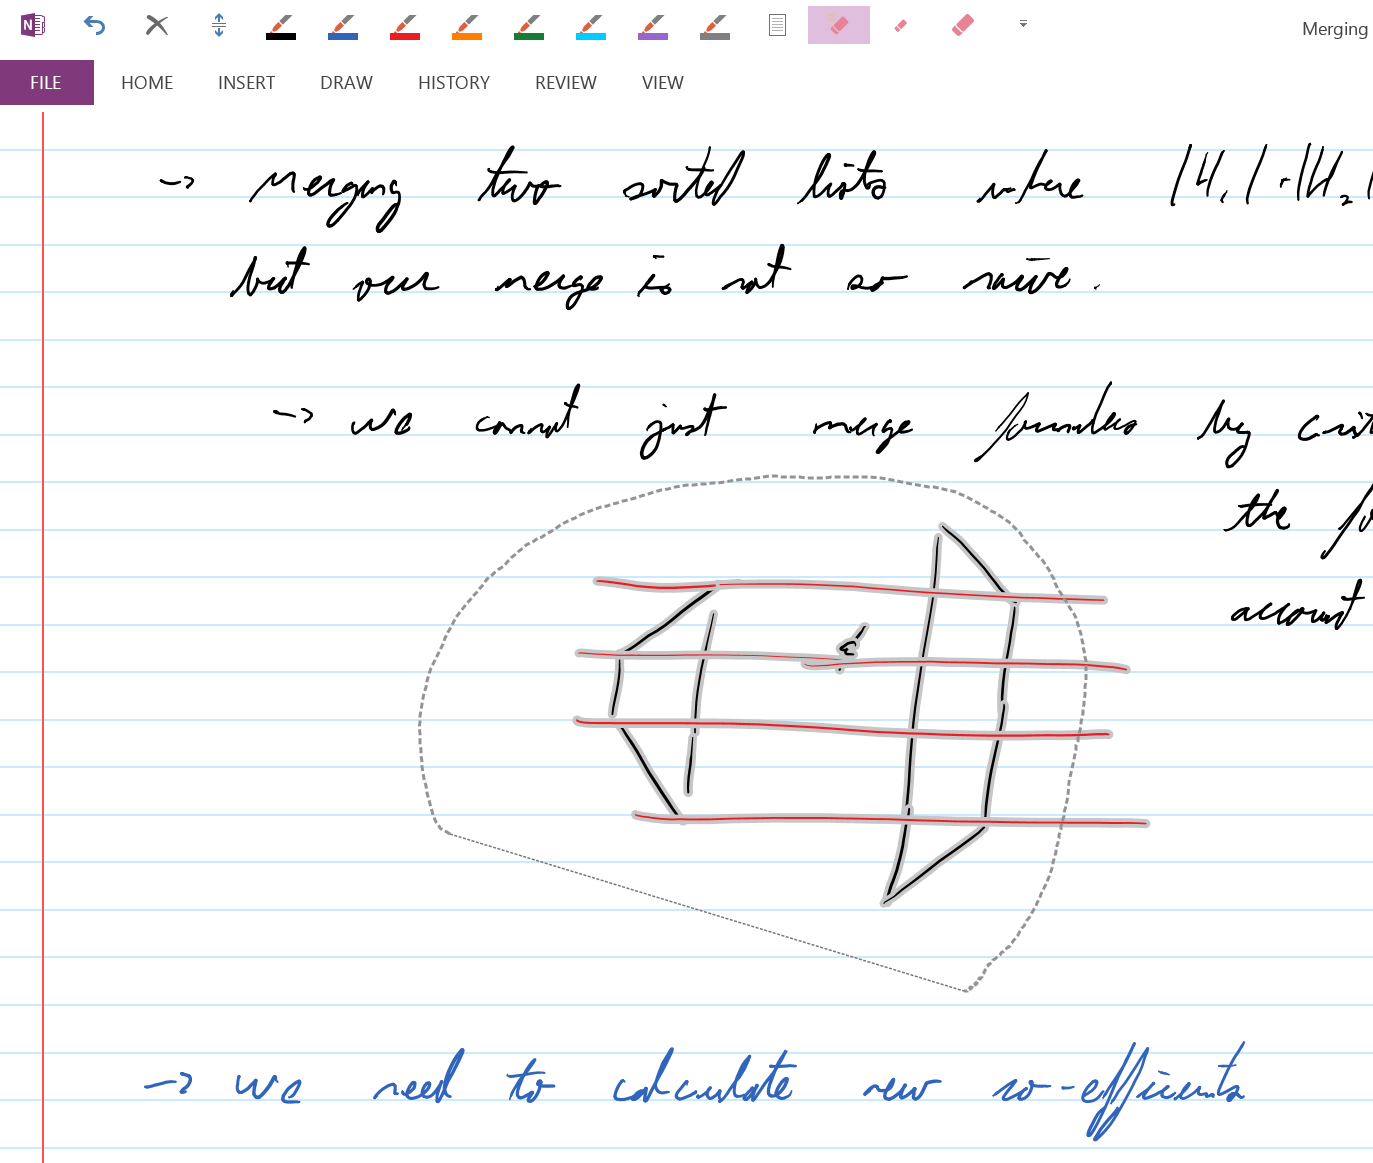
\includegraphics[width=0.50\textwidth]{figures/fig_onenote}
  \caption[An example of practical partial enclosure range searching]{An example of practical partial enclosure range searching in Microsoft OneNote. The line segments in the middle are selected even though they are not entirely enclosed.}
  \label{fig:intro:onenote}
\end{center}
\end{figure}

Looking carefully at the figure, we can see that even though the horizontal line segments of the diagram have not been entirely enclosed by the selection tool, they nevertheless appear as part of the set of selected items.
This behaviour of selecting partially enclosed objects is described in a patent filed by Microsoft Corporation\cite{lassoselect}. 
From the patent:

\begin{quote}
[T]here is a need for a selection tool that will allow a user to conveniently select one or more graphical objects in their entirety, without requiring an inconvenient amount of precision from the user.
\end{quote}

\noindent With the rising popularity of touch and pen-enabled devices, this need is likely to increase.  
As we can see from the figure, OneNote already includes an implementation of a partial selection tool like the one described by the patent. 
Although the details of the implementation are proprietary, it becomes apparent while using the software that it suffers from poor performance as more items are selected.
It is from this observation that the work in this thesis was inspired.  
Although the problems that we will examine take place in simpler settings than the patent describes, we will nevertheless develop an understanding of the major challenges of this problem domain, as well as some techniques for addressing them.


%------------------------------------------------------------------------------
%------------------------------------------------------------------------------
\section{Problem Statements}
\label{:intro:problems}

This thesis proposes algorithms for several different partial enclosure range search settings.  Each problem addresses a different type of geometric object to be queried, or a different type of query region.

\paragraph{Line Segments and Query Rectangles.} Line segments and rectangles are one of the simplest settings in which we can perform partial enclosure range searches. 
Given an axis-parallel query rectangle, we address methods which consider only axis-parallel segments, or which consider arbitrarily-oriented ones.

\paragraph{Line Segments and Query Slabs.} Relaxing the axis-parallel query regions of the preceding problem, we consider an arbitrarily-oriented slab.
As the query slab can have any orientation, intersections with a horizontal segment will involve both the height of the segment and the slope of the slab.  
We also consider a query defined as the intersection of two slabs.

\paragraph{Convex Polygons and Query Rectangles.} Moving away from line segments, we consider problems of partial enclosure with respect to area.  
For any such problem, deciding on the partial enclosure property is straight-forward once we know the area of the input object and the area enclosed by a query region.  
We consider how to determine what proportion of a convex polygon is enclosed by a rectangular query.
 
\paragraph{Monotone Polygons and Query Rectangles.} This more complex shape does not generally decompose into big convex regions, so a different method of preprocessing will be needed.
We consider methods for calculating the area of the polygon to one side of a query line. 
With such a method in hand, determining the area of a rectangle is a matter of executing several queries and combining their results.

%------------------------------------------------------------------------------
%------------------------------------------------------------------------------
\section{Related Work}
\label{:intro:related}

In this section, we review some existing variations of the range searching problem.
As a whole, due to its applicability to such a wide assortment of problems, range searching has received a great deal of research attention.
Aside from the solutions to specific problems that this research has found, it has also resulted in a vast toolbox of observations and techniques, many of which apply to our own problem.

Range searching structures are typically constructed by subdividing the input objects, or the space in which the input objects exist, into several regions which express useful properties.
Ideally, we are able to choose these regions so that a query region will entirely contain, or not contain, most of the regions, while intersecting only a small number of them.
On those intersected regions, we continue the query on the recursively finer subdivisions stored there.\cite{Matousek93}

This recursive decomposition of the input into regions has an extremely beneficial side-effect. 
At each hierarchical region, we can associate any other structure of our choosing.
These so-called multi-level structures can be used to answer complex queries by identifying objects which satisfy one property with respect to the outer structure, and then continuing with the associated structures to satisfy additional properties.
We discuss examples of this type of multi-level query in detail in Chapter~\ref{:prelim}.

The remainder of this section gives a brief introduction to some specific range searching problems, and history of some methods for answering each. 
We refer the reader to an excellent survey on range searching by Agarwal and Erickson\cite{Agarwal99} for a more detailed introduction.


\subsection*{Orthogonal Range Searching} 

In its general form, an orthogonal range searching problem starts with a set $S$ of points in $\mathbb{R}^d$, where $d$ is a small, fixed constant.
A query is a $d$-dimensional, axis-parallel box, and our goal is to identify the subset of our input points which are contained within this box.

\emph{Quadtrees}, first described by Finkel and Bentley\cite{Finkel74} (see also \cite[Chapter~14]{deberg}), are one of the very first structures for performing range searches.
When we are considering points in the plane, a quadtree works by dividing the space containing the points into squares, and then recursively splitting any region which contains more than one point into four smaller, but equally-sized squares.

Because this recursion is based on splitting space rather than the points within the space, the recursion depth, and thus the depth of the quadtree, is not related to the number of points. 
Instead, the size of the initial square from which we start splitting and the distance between the closest pair of points are the important factors.
For an initial square with a side length of $s$ and a closest pair with distance $c$, the recursion depth is $\BigOh{\log{\frac{s}{c}} + \frac{3}{2}}$.
The construction and query times are related to this recursion depth, making the structure somewhat slow, but it \emph{does} work!

Quadtrees can be easily extended to work in higher dimensions. 
In $\mathbb{R}^3$ quadtrees are called \emph{Octrees}, and the general method can be extended to even higher dimensions. 
For points and an initial box in $\mathbb{R}^d$, decomposition proceeds along the same basic rules, but using progressively smaller $d$-boxes instead of just squares.


KD-Trees\cite{Bentley75} were the first major improvement over quadtrees.
Unlike a quadtree which partitions space, a KD-Tree directly partitions the pointset in a recursive manner.
For points in the plane, each level of the tree corresponds to a particular axis.
Suppose that we start with the $x$-axis at the root level.
We consider the median point $m$ with respect to the $x$-coordinates of all the points, and then all remaining points are partitioned as left or right of this vertical \emph{splitting line} through $m$.

On the next level of the recursion we alternate to the $y$-axis, select the median point with respect to $y$-coordinates, and partition around the horizontal splitting line through that point.
The process continues, alternating the axis on each level, until we create leaves containing single points.
This process creates a balanced tree, where each path through the tree alternates between axes.
Each node in the tree represents a region of the plane bounded by its own splitting line and the splitting lines of its ancestors.

Querying a KD-Tree by a rectangular region involves traversing the tree while only visiting those nodes whose region is intersected by the query region.
While the preprocessing requirements of a KD-Tree are quite good, at $\BigOh{n}$ space and $\BigOh{n\log{n}}$ preprocessing time, the query time is $\BigOh{\sqrt{n}}$.

A final note about KD-trees, this recursive construction can be generalized to higher dimensions in a straight-forward manner, by simply cycling through each of the $d$ axes in order.
The preprocessing requirements are unchanged asymptotically, since we still create just a single binary tree with $n$ leaves.
The query algorithm is also similar to the $\mathbb{R}^2$ case, but with a query time of $\BigOh{n^{1-1/d}}$.

The next improvement in orthogonal range searching came in the form of a polylogarithmic method known as \emph{Range Trees}. 
Range trees were discovered by Bentley\cite{Bentley79}, who was involved in the last two structures, but were also simultaneously developed by other independent researchers.
This method is constructed on binary search trees and can query any open or closed query box in $\BigOh{\log^{d-1}{n}}$ time with only $\BigOh{\log^{d-1}{n}}$ time and space pre-processing.
We discuss this structure in more detail in Section~\ref{:prelim:range-trees}.

%Best known by Chazelle [Dutch 90,91] in 2D and higher dimensions with time/space of XXX

Finally, a noteworthy special case occurs when our points are in the plane and our query is a three-sided rectangle, i.e., when it is open to one side.
In this case, we can use a method developed by McCreight\cite{McCreight85} which gives $\BigOh{\log{n}}$ query time while using only $\BigOh{n}$ space and $\BigOh{n\log{n}}$ preprocessing time.

The real power of orthogonal range searching is in how other problems can be reduced to instances of it by encoding query keys as coordinates of a high-dimensional point.  
For example, in the geometric sense, we can search for rectangles inside of rectangles by mapping the coordinates of an input rectangle in $\mathcal{R}^{d}$ to a point in $\mathcal{R}^{2d}$, and performing an orthogonal range search in that space.
Rectangle-in-rectangle queries are important as rectangles make easy approximations of more complicated geometric objects that we may want to look for.

Outside of purely geometric applications, many more general types of range searching problems can be reduced to instances of orthogonal range searching by encoding query keys as coordinates of a high-dimensional point.
For example, given some integer representation of a date, we can search for emails received within a date range by encoding the date stamp of each email into a point, and then searching for points between the two integer representations of our query range.
Extending this idea to more complex queries is just a matter of mapping each key we wish to search on to further components of a higher-dimensional point.  
In this way, multi-dimensional orthogonal range searching can be used to perform multi-key searching.\cite{Willard96} 


\subsection*{Half-plane Range Searching}

In general, when performing half-plane queries, we need to make a choice between using a structure which has low space or one with a fast (polylogarithmic) query time.
We introduce a structure suitable for each side of this trade-off.

If we want to save space, we can use a \emph{Ham Sandwich Cut Tree}\cite{Edelsbrunner86, Edelsbrunner87}.
To construct this tree, we divide all of our points into four quadrants of equal size, which we accomplish with an algorithm by Megiddo\cite{Megiddo85} in $\BigOh{n}$ time.
We continue construction by repeating this process on each quadrant recursively, and building a tree out of the results of each step.
The final tree has size $\BigOh{n}$ and is constructed in $\BigOh{n\log{n}}$ time.

We can query this tree with the line representing the boundary of a query half-plane.
The quadrants at any step are the result of two intersecting lines, and thus, our query line will intersect at most three of them.
The non-intersected quadrants, of which there is at least one, are entirely inside the query half-plane, or entirely outside of it.
The query then recurses on the intersected quadrants.
Total query time is $\BigOh{n^{\log_2(1 + \sqrt{5}) - 1}} \approx \BigOh{n^{0.695}}$.


If we want to save query time, then we can use a \emph{Level Arrangement}\cite{GoswamiDN04}.  
This structure has a query time of only $\BigOh{\log{n}}$ but requires $\BigOh{n^2}$ storage.
The level arrangement structure is constructed in a dual space.
Given a set $S$ of $n$ points $p_1, p_2, \ldots, p_n$ where each $p_i = (a_i, b_i)$, we map each point to a corresponding dual line $l_i: y = a_i \cdot x - b_i$.

Considering all of the intersection points formed by the set of dual lines crossing each other, and the edges between them, we can easily see the $\BigOh{n^2}$ size.
Preprocessing continues by enclosing the environment in a bounding box which contains all of the intersections.
By following the monotone chains of intersections from left to right, we can determine the ``level'' of each edge, that is, the number of edges below (or above) each edge.
Total preprocessing time is $\BigOh{n^2}$.

In this dual space, the line which defines the boundary to our query half-plane becomes mapped to a point.
The query proceeds by selecting the median level of the arrangement, and then performing a binary search over its edges to find the one above or below the query point.
This process is repeated in a binary search sort of fashion on the subset of levels containing the query point until we have found the levels directly above and below the query point. 
Depending on the half-plane, the levels lying to one side of the query point or the other correspond to the input points satisfying the query half-plane.
As we have described it here, this query requires $\BigOh{\log^2{n}}$ time, but this can be reduced to $\BigOh{\log{n}}$.\cite{NandyDG03}

A different approach to solving half-plane range searches altogether is to consider a half-plane as a degenerate simplex, and then use any simplex range searching structure to answer a query.  
Such structures are discussed below and in Section~\ref{:prelim:chan}.

One final method for half-plane searches we would like to mention is by Chazelle \emph{et al.}\cite{ChazelleGL85,Chazelle85} as it does not obey the general trade-off between space and query time that we mentioned above.
This method uses \emph{convex layers} and gives both $\BigOh{n}$ storage and $\BigOh{\log{n} + k}$ query time, where $k$ is the number of elements reported. 
However, this method can only be used for reporting queries, and is not well suited to counting or multi-level queries.

Convex layers of a pointset are easiest to explain by their construction, which is performed iteratively by calculating the convex hull, deleting it, and then taking the convex hull of what remains, until all points are deleted.
Convex layers can be constructed in $\BigOh{n\log{n}}$ time, and require $\BigOh{n}$ space.
In order to use convex layers for half-plane queries, we will translate the pointset such that the origin point of the plane occurs inside the innermost layer.

A query line which passes through the pointset will intersect some or all of the layers, from $l_1$ at the outside to $l_m$, the innermost layer which is intersected.
The query is performed in two main steps: identify $l_m$, and then report all of the points.

Locating $l_m$ is done in a dual space transformation.
Our pointset becomes an arrangement of lines, and our query line becomes a point.
A consequence of the origin point being inside the innermost convex layer in the primal space is that the dual space will be comprised of corresponding levels, although in reverse order.
We can then perform any planar point location method we like on the query point to determine the level containing it; Chazelle \emph{et al.} give several $\BigOh{\log{n}}$ choices.

With the convex layer $l_m$ known, we can compute the intersections of the query line with $l_m$ in $\BigOh{\log{n}}$ time, and in so doing, identify at least one point which is inside our query half-plane.
During processing, we augment every vertex with pointers to the edges which appear above and below them in neighbouring convex layers, accomplished by walking around two neighbouring layers at a time simultaneously.
Depending on which side of the query line our half-plane extends, we can walk these pointers from $l_m$ across the remaining levels, whether that first takes us deeper into the layers, or directly out.
At each level, we then traverse left and right around the level for as long as we remain in the query half-plane reporting our matching points.


\subsection*{Simplex Range Searching}

In simplex range searching in the plane, there is no known data structure which can answer a query in polylogarithmic time using linear (or nearly linear) storage.\cite{Agarwal99}  

Considering structures with linear or near linear storage, the first sublinear query time algorithm in this area was by Willard in 1982\cite{Willard82}.
His paper introduced a method using \emph{partition trees}.
The general idea is to partition space into several regions each containing a roughly equal number of input points.
Each region is then recursively built in the same way.
The goal is to choose our regions in such a way that the largest number of regions which may be intersected by any line is minimized.  
This property is known as the \emph{crossing number}.
Willard's approach requires a query time of $\BigOh{n^{0.774}}$.
Moreover, the partition tree approach in general expresses a ``nice'' recursive structure which lends itself to multi-level query structures.

Following this first approach, a series of improvements were made to the partition tree method, mostly concentrating on developing a lower crossing number.
For many years, the best known approach was by Matousek\cite{Matousek92} which requires $\BigOh{n\log{n}}$ preprocessing time and $\BigOh{\sqrt{n}\log^{\BigOh{1}}{n}}$ query time.
Recently, this has been improved to a query time of just $\BigOh{\sqrt{n}}$ by Chan\cite{chan2012} with the same preprocessing time.
We use this latter method throughout Chapters \ref{:rectangles} and \ref{:slabs}, and discuss it in more detail in Section~\ref{:prelim:chan}.


\subsection*{Intersection Searching} 

Intersection searching is similar to range searching, except that we consider different types of geometric input objects aside from points.
Given a query region, we are looking for any objects which have even a single point of intersection in common with the query itself; that is, the object need not be entirely enclosed with the query region.
In this way, we can think of range searching as a specialization of intersection searching.
There are many variations of intersection searching, of which we introduce a few.

In \emph{Segment Intersection Searching}, the query range is a line segment. 
If both the input objects and the query range are segments, 

\emph{Rectangle Intersection Searching}, also known as \emph{Windowing Queries} identify polygons which intersect a rectangular query region. 
Many computer graphics problems are related to this problem as, for example, we might want to determine what items need to be rendered on screen from a 3D environment.

Finally, \emph{Point Intersection Searching} is sort of the opposite of an normal range searching query. In this problem, we are interested in reporting all objects which contain a query point.


\subsection*{Completing a Search}

Throughout this section, we've used the term ``identify'' rather loosely.
For the hierarchical structures above, ``identifying'' points satisfying a query really comes down to isolating those partitions which contain them.
What we do with them at that point is somewhat flexible.
For example, we can simply count the points we have identified with only a constant factor of extra time and space by having the partitions store their own sizes.
We could instead report the points by traversing each terminal of the partition, which will cost us an extra linear factor with respect to to the number of reported items.

We conclude this section by comparing and contrasting our own problem with the ones we have just introduced.

Our problem is notably different from standard range searching problems because we are not just looking for items which are entirely contained inside of a query region.
This immediately rules out a simple application of orthogonal range searching like we saw with the rectangles-in-rectangles problems.

Our problem differs from intersection searching as well, since we have the extra constraint of requiring a specific proportion of the input objects to be contained in the query region, rather than just any point.


%------------------------------------------------------------------------------
%------------------------------------------------------------------------------
\section{Summary of Contributions}
\label{:intro:contributions}

In this thesis, we develop contributions to several variations of the \PERS{} problem, along with some noteworthy ancillary methods. 
Table~\ref{tab:contributions} gives a broad overview of the data structures we develop. 
The table uses `AP' for ``Axis-Parallel'', `AO' for ``Arbitrary Orientation'', and `P' for ``Polygon'', and omits ``Big Oh'' for clarity.

\begin{table}[t]
\caption{Summary of Contributions}
\label{tab:contributions}
\centering
\begin{tabular}{l l l l l l}
\hline \hline
Object & Query & Theorem & Space & Time & Query \\
\hline
AP Segment & AP Rectangle & Th~\ref{th:ap} & ${n\log^3{n}}$ & ${n\log^3{n}}$ & ${\log^3{n}}$ \\
AO Segment & AP Rectangle & Th~\ref{th:ao} & ${n\log^7{n}}$ & ${n\log^7{n}}$ & ${\sqrt{n}\log^7{n}}$ \\
AP Segment & AO Slab & Th~\ref{th:slabs:one} & ${n\log^2{n}}$ & ${n\log^3{n}}$ & ${\sqrt{n}\log^3{n}}$ \\
AP Segment & 2 AO Slabs & Th~\ref{th:slabs:two} & ${n\log^3{n}}$ & ${n\log^3{n}}$ & ${\sqrt{n}\log^3{n}}$ \\
Convex P & Rectangle & Th~\ref{th:convexp:area} & ${n}$ & ${n}$ & ${\log{n}}$ \\
Convex P & Convex $k$-gon & Cor~\ref{cor:convexp:karea} & ${n}$ & ${n}$ & ${k \log{n}}$ \\
Monotone P & AP Rectangle & Th~\ref{th:monotonep:rect:area} & ${n\log{n}}$ & ${n\log{n}}$ & ${\log{n}}$ \\
Monotone P & AP Rectangle & Th~\ref{th:mono2} & ${n}$ & ${n\log{n}}$ & ${\sqrt{n}}$ \\
Simple P & Horiz Slab & Cor~\ref{cor:monotonep:simplep-area} & ${n}$ & ${n}$ & ${\log{n}}$ \\
\hline
\end{tabular}
\end{table}

In the line segment cases, we develop methods for restating the partial enclosure property as something which can be evaluated as a one or two variable inequality. 
These expressions can then be queried by known structures for orthogonal or half-plane queries. 
We discuss the transformations to appropriate dual-spaces and the design of data structures which can answer the necessary multi-part queries.

In the polygon cases, we primarily develop methods for calculating area within a simple region, e.g., below a query line.
These methods are then repeated and combined to find the area enclosed by the actual query region.
Once the enclosed area is known, determining the partial enclosure property is straight-forward.

%------------------------------------------------------------------------------
%------------------------------------------------------------------------------
\section{Organization of the Thesis}
\label{:intro:organization}

The remainder of this thesis is organized in the following way. 
Chapter~\ref{:prelim} reviews existing data structures and range searching techniques which we utilize in our own contributions.
The next four chapters cover partial enclosure range searching queries on successively more sophisticated geometric objects, with Chapter~\ref{:rectangles} focusing on axis-parallel rectangles, Chapter~\ref{:slabs} on arbitrarily-oriented slabs, Chapter~\ref{:convexp} on convex polygons, and Chapter~\ref{:monotonep} on monotone polygons.
The thesis concludes with Chapter~\ref{:conclusion} which summarizes the contributions and future work presented in earlier chapters.

\chapter{Preliminaries}
\label{:prelim}

In this chapter, we outline the data structures and other techniques which we rely on for the formulation of solutions to our own contributions.

%------------------------------------------------------------------------------
\section{Range Trees}
\label{:prelim:range-trees}

A range tree is a binary search tree that allows us to search for elements satisfying a 1D query interval. Given a set of $n$ elements, $A = \{a_1, a_2, \ldots, a_n\}$, each expressing a scalar key value $v_1, v_2, \ldots, v_n$, a range tree $T$ can identify the elements whose key falls between two values $\alpha$ and $\beta$, where $\alpha \leq \beta$.  That is, the search identified the following set:
\[
\{ a_i \in A \st \alpha \leq v_i \leq \beta \}
\]

This search can be done in $\BigOh{\log{n}}$ time with only $\BigOh{n}$ space and $\BigOh{n\log{n}}$ pre-processing time.  Reporting the matching elements can be done in $\BigOh{\log{n} + k}$ time, where $k$ is the number of elements reported. 

However, all of these properties are also true of a regular binary search on a sorted array, so why are range trees interesting? To answer this, we look at a simple example of a range tree. Suppose $A$ is a set of 2D points embedded in the plane, and that, for our query, we wish to identify all points whose $x$-coordinate is between $\alpha$ and $\beta$.  To answer this query, we can construct a range tree $T$ where each point $a_i$, $1 \leq i \leq n$ is represented by leaf node whose key value is set to the $x$-coordinate of $a_i$; that is, where $v_i = a_i.x$.

When we query $T$ for $\alpha$ and $\beta$, we identify two paths through $T$ in $\BigOh{\log{n}}$ time. The leaf with key value $\alpha$ (or with the successor value to $\alpha$, if the exact value is not present) is $a_\alpha$ and is the leftmost point in $A$ matching our query.  Similarly, the leaf with key value $\beta$ (or with the  predecessor to $\beta$, if the exact value is not present) is $a_\beta$ and is the rightmost point in $A$ matching our query. Since the leaves in a binary search tree are sorted, the sequence of points from $a_\alpha$ to $a_\beta$ are exactly the points we need to identify. We can report these points with an inorder traversal.

\begin{figure}
\begin{center}
  \includegraphics[width=0.40\textwidth]{figures/fig_pre_range1d}
  \caption{A 1D range tree and the subtrees identified by a query.}
  \label{fig:pre:range1d}
\end{center}
\end{figure}

What makes range trees such versatile structures is not simply that they identify the query elements, but rather due to the way that they group the identified elements into at most $\BigOh{\log{n}}$ disjoint subsets. These subsets are precisely the elements found in the ``inner'' subtrees along the path from $a_\alpha$ to $a_\beta$, as illustrated in Figure~\ref{fig:pre:range1d}.

With each non-leaf node of $T$, we can store additional information about the subset represented by its subtree.  The, during query time, we only need to consider the information stored at $\BigOh{\log{n}}$ nodes rather than the $\BigOh{n}$ elements they represent. Continuing our example on 2D points, with only $\BigOh{1}$ extra space per node, we could store which point has the highest $y$-coordinate in each subtree.  Then, we can use our range tree to find the highest point between two $x$-coordinates in $\BigOh{\log{n}}$ time.

We are not limited to just storing simple values with each node, however. With each node, we can associate an entire additional data structure, constructed on the elements represented by that node. In particular, we can store another range tree which is based on some other property of each element.  When we query this two-level range tree, our query at the first level identifies $\BigOh{\log{n}}$ subsets. Each subset represents elements which satisfy a particular query condition. Then, for each subset, we query the associated data structure to identify elements satisfying a second query condition.  The elements identified here satisfy both conditions. This technique can be repeated to create \emph{multi-level range trees} with more than just two levels.

The following theorems on range trees, restated from \cite{debergch5}, detail the construction and query times of multi-level range trees.

\begin{theorem}
\label{th:rangetree}
Let $P$ be a set of $n$ points in $d$-dimensional space, with $d \geq 2$. A multi-level range tree for $P$ uses $\BigOh{n \log^{d-1}{n}}$ storage and it can be constructed in $\BigOh{n \log^{d-1}{n}}$ time. With this range tree one can report the points in $P$ that lie in a rectangular query range in $\BigOh{\log^{d-1}{n} + k}$ time where $k$ is the number of reported points.
\end{theorem}

If each node of the range tree is augmented with information about the size of its subtree, then we can count the number of items within a query rectangle rather than reporting them. The following corollary summarizes this.

\begin{corollary}
\label{cor:rangetree}
Let $P$ be a set of $n$ points in $d$-dimensional space, with $d \geq 2$. A multi-level range tree for $P$ uses $\BigOh{n \log^{d-1}{n}}$ storage and it can be constructed in $\BigOh{n \log^{d-1}{n}}$ time. With this range tree one can count the points in $P$ that lie in a rectangular query range in $\BigOh{\log^{d-1}{n}}$ time.
\end{corollary}


%------------------------------------------------------------------------------
\section{Canonical Subsets Data Structure}
\label{:prelim:chan}

XXX TODO

Restated with $d=2$.

\begin{theorem}[Corollary 7.3, part $i$, in Chan\cite{chan2012}]
\label{th:chan}
We can form $\BigOh{n}$ canonical subsets of total size $\BigOh{n \log{n}}$ in $\BigOh{n \log{n}}$ time, such that the subset of all points inside any query simplex can be reported as a union of disjoint canonical subsets $C_i$ with $\sum_i{\sqrt{|C_i|}} \leq \BigOh{\sqrt{n}\log{n}}$ in time $\BigOh{\sqrt{n}\log{n}}$ w.h.p. $(n)$.
\end{theorem}

This structure is particularly well-suited to multi-level query structures, as we can associate additional data structures with each of the canonical subsets.

\begin{corollary}
\label{cor:multichan}
With each of the $k = \BigOh{n}$ canonical subsets $C_1, C_2, \ldots, C_k$ created for a canonical subsets structure, we can associate a data structure with the elements of each subset. 
Let this associated structure require $\BigOh{m\log^f{m}}$ preprocessing space, $\BigOh{m \log^g{m}}$ preprocessing time, and $\BigOh{\sqrt{m}\log^h{m}}$ query time, where $f, g, h \in \BigOh{1}, f \leq g$, and $m$ the number of elements it is constructed on. 
The resulting multi-level data structure requires $\BigOh{n\log^{f+1}{n}}$ preprocessing space, $\BigOh{n\log^{g+1}{n}}$ preprocessing time, and $\BigOh{\sqrt{n}\log^{h+1}{n}}$ query time.
\end{corollary}

\begin{proof}
The preprocessing space of the multi-level structure requires $\BigOh{n \log{n}}$ space for the canonical subsets structure itself, plus
\[
\begin{split}
\sum_{i=1}^k{|C_i| \log^f{|C_i|}}
&\leq \sum_{i=1}^k{|C_i| \log^f{n}} \\
%
&\leq \BigOh{\log^f{n}} \cdot \sum_{i=1}^k{|C_i|} \\
%
&\leq \BigOh{n\log^{f+1}{n}}
\end{split}
\]

\noindent for the associate structures, for a total space complexity of $\BigOh{n \log{n}} + \BigOh{n\log^{f+1}{n}} = \BigOh{n\log^{f+1}{n}}$.

Preprocessing time is calculated using similar reasoning, and includes the $\BigOh{n \log{n}}$ time for building the canonical subsets structure itself, plus
\[
\begin{split}
\sum_{i=1}^k{|C_i| \log^g{|C_i|}}
&\leq \sum_{i=1}^k{|C_i| \log^g{n}} \\
%
&\leq \BigOh{\log^g{n}} \cdot \sum_{i=1}^k{|C_i|} \\
%
&\leq \BigOh{n\log^{g+1}{n}}
\end{split}
\]

\noindent for building the associate structures, for a total time complexity of $\BigOh{n \log{n}} + \BigOh{n\log^{g+1}{n}} = \BigOh{n\log^{g+1}{n}}$.

Querying requires $\BigOh{\sqrt{n}\log{n}}$ time to find the $k'$ disjoint canonical subsets representing the elements found by the top-level canonical subsets query, plus
\[
\begin{split}
\sum_{i=1}^{k'}{\BigOh{\sqrt{|C_i|}\log^h{|C_i|}}} 
&\leq \sum_{i=1}^{k'}{\BigOh{\sqrt{|C_i|}\log^h{n}}} \\
%
&\leq \BigOh{\log^h{n}} \cdot \sum_{i=1}^{k'}{\BigOh{\sqrt{|C_i|}}} \\
%
&\leq \BigOh{\sqrt{n}\log^{h+1}{n}} \\
\end{split}
\]

\noindent to query all of the appropriate associated data structures, for a total query time of 
\[
\BigOh{\sqrt{n}\log{n}} + \BigOh{\sqrt{n}\log^{h+1}{n}} = \BigOh{\sqrt{n}\log^{h+1}{n}}
\]

\end{proof}

An example of how we can use a multi-level canonical subsets structure is as follows. 
Suppose we have $n$ line segments in the plane.
Each line segment $s_i$, $1 \leq i \leq n$ is given by its left endpoint $p_i = (a_i, b_i)$ and its right endpoint $q_i = (c_i, d_i)$.
We would like to identify all segments intersected by a query line $L: y = \alpha x + \beta$.

We will solve this query in two steps, by first identifying all segments whose left endpoint is left of $L$. 
Of those, we will then identify which have their right endpoint right of $L$.
Describing the construction of a multi-level data structure is often clearer when we begin with the innermost level.
With that in mind, we consider the right endpoints first. 
Considering only the points $q_i$, $1 \leq i \leq n$, and using $L$ to define a half-plane, we apply 
Theorem~\ref{th:chan} to create a structure in $\BigOh{n\log{n}}$ time and space which will identify all points inside the half-plane in $\BigOh{\sqrt{n}\log{n}}$ time.  While each subset in this structure is ``keyed'' on right-endpoints, we can store the line segments as well.

Considering the left endpoints now, applying Theorem~\ref{th:chan} again gives us another structure with identical preprocessing and query times.  On this structure, however, we will associate an instance of the structure from step 1 with every subset, constructed on only the elements from its respective subset. By Corollary~\ref{cor:multichan}, this multi-level data structure will require $\BigOh{n\log^2{n}}$ time and space, and will identify all segments whose left endpoint is left of $L$ \emph{and} whose right endpoint is right of $L$ in $\BigOh{\sqrt{n}\log^2{n}}$ time.

\chapter{Majority Range Queries with Axis-Parallel Rectangles}
\label{:rectangles}

In this chapter, we begin with a simple environment for performing majority range queries. Even with this simplified model, we will be able to identify where the main challenges of this problem domain lie and construct some techniques which we will use to solve many of the more complex problems.

We will present two variations of the majority range search problem in this chapter. Both use axis-parallel rectangles as their query. Both variations will query over line segments, which are the simplest type of object which has a concept of majority. In the first variation, the line segments will also be axis-parallel, whereas in Section~\ref{:rectangles:ao}, we allow segments of arbitrary orientation.

%------------------------------------------------------------------------------
\section{Axis-Parallel Segments}
\label{:rectangles:ap}

In this section we consider axis-parallel line segments in the plane and queries in the form of axis-parallel rectangles.
This is the simplest 2D environment on which we can perform a majority range query as the objects and query region are both simple geometric objects, and we can rely on their fixed orientations while expressing equations about them. 
We will discuss only horizontal segments here.
The solution for vertical segments is identical, and we discuss how to combine the two approaches at the end of the section.

We define our first problem as follows.

\begin{problem}
Given a set $S$ of $n$ axis-parallel line segments in the plane, and a fixed parameter $\rho$ such that $0 < \rho \leq 1$, we want to return the number of segments from $S$ which are mostly enclosed by an axis-parallel query rectangle $Q$. A given segment $s \in S$ satisfies the majority property (i.e., is considered mostly enclosed by $Q$) if and only if $|s \cap Q| \geq \rho \cdot |s|$.
\end{problem}


\subsection{Definitions}
\label{:rectangles:ap:defs}

Each segment $s_i \in S, 1 \leq i \leq n$ is defined by its two endpoints $p_i = (a_i, b_i)$ and $q_i = (c_i, d_i)$. 
Without loss of generality, we will assume that $p_i$ is the leftmost endpoint of $s_i$ (or the lower endpoint if $s_i$ is vertical). 
We define $l_i = |s_i|$ as the length of $s_i$; for horizontal segments the length is easily calculated as $l_i = c_i - a_i$. 
Our query $Q$ is given by its lower-left corner $(\alpha, \beta)$ and its upper-right corner $(\gamma, \delta)$. 
$s_i \in_\rho Q$ if $s_i$ satisfies the majority property for $Q$, otherwise $s \not \in_\rho Q$.

For any $x$-coordinate, $\iline{x}$ is the vertical line through $x$. Similarly, for any $y$-coordinate, $\iline{y}$ is the horizontal line through $y$. For example, $\iline{\beta}$ is the horizontal line through the bottom boundary of $Q$, while $\iline{a_i}$ is the vertical line through $a_i$, and thus, through the left endpoint of $s_i$. Finally, we define $\iline{s_i}$ as the line through the segment $s_i$; for a horizontal segment $s_i$, the lines $\iline{s_i}$, $\iline{b_i}$, and $\iline{d_i}$ are all equivalent. When we focus on any single, general segment, we omit the $i$ subscripts for clarity.


\subsection{Decomposing the Problem}
\label{:rectangles:ap:approach}

\begin{figure}[t]
\centering
\includegraphics[width=1.00\columnwidth]{figures/fig_oo_cases}
\caption[The different cases of axis-parallel segments.]{An axis-parallel query on axis-parallel segments. Different cases of horizontal segments interacting with the query region are shown.}
\label{:fig:rectangles:ap:cases}
\end{figure}

As Figure~\ref{:fig:rectangles:ap:cases} illustrates, there are several cases to consider regarding how a horizontal segment $s \in S$ may interact with $Q$. Cases $(1)$, $(2)$, and $(3)$, where $s$ is entirely left, entirely within, or entirely right of $Q$, respectively, are exactly an instance of  standard range searching problems where we look to find elements which are completely inside or completely outside of a query region.  

Case $(4)$ considers segments where $s$ crosses only the left boundary of $Q$. 
Looking at it another way, $s$ has its left endpoint left of $\alpha$, while its right endpoint $q$ satisfies $\alpha \leq q \leq \gamma$.  
We further subdivide case $(4)$ into cases where, for some appropriate value of $\rho$, $s \in_\rho Q$ in case $(4a)$ and $s \not \in_\rho Q$ in case $(4b)$.
Cases $(5a)$ and $(5b)$ are similar to cases $(4a)$ and $(4b)$, but with respect to $\gamma$. 
Specifically, $s$ falls into case $(5)$ when $\alpha \leq p \leq \gamma$ and $q > \gamma$. 

In case $(6)$, $s$ crosses both the left and right boundaries of $Q$, and, crucially, neither $p$ nor $q$ are inside $Q$. As like in cases $(4)$ and $(5)$, $s$ is in case $(6a)$ if $s \in_\rho Q$ and $(6b)$ if $s \not \in_\rho Q$.

Our goal is to identify and count all of the segments belonging to cases $(2)$, $(4a)$, $(5a)$, and $(6a)$, and none of the segments belonging to any other case.

Our approach to solving this problem involves restricting and classifying segments step-by-step until, for some subset of segments, we are able to identify an expression representing its majority property.  Our solution proceeds as follows.

\paragraph{Step 1.} As we are only considering horizontal segments for now, we only need to consider those segments which are neither above nor below $Q$, since they can never intersect $Q$ at all. Let $S_1 = \{ s \in S \st \beta \leq b \leq \delta\}$. 

\paragraph{Step 2.} We identify those segments which are not ``too long''.  Let $w = \gamma - \alpha$ be the width of $Q$.  Any segment $s$ having the property $|s| > \frac{w}{\rho}$ can never have its majority property satisfied, no matter how it intersects $Q$.  Let $S_2 = \{ s \in S_1 \st |s| \leq \frac{w}{\rho} \}$.

\paragraph{Step 3.} We partition the remaining segments according the location of their left endpoint with respect to $\alpha$.
Specifically, let $S_L = \{s \in S_2 \st a < \alpha \}$ and let $S_R = \{ s \in S_2 \st a \geq \alpha \}$.

\paragraph{Step 4.} We test the appropriate majority expression to determine if $s$ should be counted. For segments whose left endpoint is left of $\alpha$, we want to ensure that ``not too much of $s$ is outside of $Q$''; Let $S_L' = \{ s \in S_L \st \alpha - a < (1 - \rho) \cdot l\}$. For segments whose left endpoint is at or right of $\alpha$, we want to ensure that ``enough of $s$ is inside $Q$''; Let $S_R' = \{ s \in S_R \st \gamma - a \geq  \rho l \}$. Our claim is that the subset of segments satisfying the majority property is $S_\rho = S_L' \cup S_R'$. 

\begin{proof}
The correctness of Steps 1 and 2 are straight-forward, and Step 3 merely partitions the remaining segments. Thus, we focus on Step 4 and show that for each case, a segment belonging to that case is correctly accepted or rejected.

Consider the segments in $S_L$, which we check against the majority property expression $\alpha - a < (1 - \rho) \cdot l$. That is, we are looking at how much of $s$ is outside of $Q$. Segments in case $(1)$ have $\alpha - a > l$, so they are correctly rejected. Segments in cases $(4a)$ and $(4b)$ are accepted or rejected quite straight-forwardly by this condition; that is, if not too much of $s$ is outside $Q$, then ``enough'' of $s$ must be inside.  

The most interesting cases are $(6a)$ and $(6b)$, and they are the motivation behind Step 2.  After Step 2, we know that $|s| < \frac{w}{\rho}$, which implies that any segment in $s \in S_L$ that crosses both $\alpha$ and $\gamma$ must satisfy $s \in_\rho Q$, since $|s \cap Q|$ is exactly $w$, and $w$ is sufficient. This property allows us to avoid explicitly deciding if $s$ crosses $\gamma$, since if not too much of $s$ is outside $Q$, $s$ either crosses only $\alpha$ and case $(4)$ holds, or it crosses $\alpha$ and $\gamma$, and $w$ is sufficient.

Next, we consider the segments in $S_R$, which we check against the majority property expression $\gamma - a \geq  \rho l$ for $s \in S_R$. 
This expression checks the affirmative case, that is, that enough of $s$ is inside $Q$.
For case $(2)$, $\gamma - a \geq l$. 
Since $l \geq \rho l$ for all valid values of $\rho$, these segments are accepted.
On the other hand, for case $(3)$, $\gamma - a < 0$ and all such segments are rejected. 
In the final cases, $(5a)$ and $(5b)$, the value of $|s \cap Q|$ is measured directly, and the segments are classified appropriately.

\end{proof}


\subsection{Construction and Analysis}
\label{:rectangles:ap:analysis}

Each step of Section~\ref{:rectangles:ap:approach} includes or excludes segments by examining inequalities. Each inequality is made up of some of the input parameters of each segment and a single query variable. To perform the query, we will map each segment to a point in 4D where each component of the point is based on the segment input parameters corresponding to one of our inequalities, and map the query variables given by $Q$ to a 4D box. The query can then be answered using a multi-level range tree.

Recall that for every $s \in S$, we have $s = (a, b, l)$ as the $x$-coordinate of the left endpoint, $y$-coordinate of the left endpoint, and length of the segment, respectively.  The query region $Q$ has width $w = \gamma - \alpha$. Let $v$ be the 4D point we create which corresponds to $s$.

The first two conditions we need to check are the same for all cases. 
We first isolate segments based directly on their $y$-coordinate; thus, the first component of $v$ will be $b$, and the first component of our 4D query box will be $[\beta, \delta]$.
We next want to include only segments where $l \leq \frac{w}{\rho}$. We can rewrite this as $\rho l \leq w$. 
Thus, the second component of $v$ will be $\rho l$, and the second component of our query box will be $(0, w]$.

Our segments are next classified according to which side of $\alpha$ their left endpoints are found.
We set the third component of $v$ to $a$.
Our overall query will need to look at both cases and combine the results later. 
The third component of the query box will be either $(-\infty, \alpha)$ or $[\alpha, \infty)$ depending on which phase of the query is executing.

Finally, we need to check the majority expressions. We have two cases to check. The first expression is for segments whose left endpoint is left of $\alpha$. The majority expression $\alpha - a < (1 - \rho) \cdot l$ can be rewritten as $\alpha < a + (1-\rho) \cdot l$. Therefore, we set the fourth component of $v$ to $a + (1 - \rho) \cdot l$, and the fourth component of the query box to $(\alpha, \infty)$.  All together, to answer this case, every segment $s_i \in S$ is mapped to the 4D point 
\[ 
v_i = (b_i, \rho l_i, a_i, a_i + (1-\rho) \cdot l_i)
\]

\noindent and is queried by the 4D query box
\[
[\beta, \delta] \times (0, w] \times (-\infty, \alpha) \times (\alpha, \infty)
\]

The second expression is for segments whose left endpoint is at or right of $\alpha$. The majority expression $\gamma - a \geq \rho l$ can be rewritten as $\gamma \geq a + \rho l$. 
Therefore, we set the fourth component of $v$ to $a + \rho l$, and the fourth component of the query box to $(-\infty, \gamma]$.  
All together, to answer this case, every segment $s_i \in S$ is mapped to the point
\[
v_i' = (b_i, \rho l_i, a_i, a_i + \rho l_i)
\]

\noindent and is queried by the box
\[
[\beta, \delta] \times (0, w] \times [\alpha, \infty) \times (-\infty, \gamma]
\]

By Corollary~\ref{cor:rangetree}, we can answer either of these queries by constructing a multi-level range tree.
As our points are in 4D, such a tree would require $\BigOh{n \log^3{n}}$ time and space for preprocessing and could answer queries in $\BigOh{\log^3{n}}$ time.
To find all horizontal segments satisfying their majority property, we need to perform both queries and combine the results.  

A second data structure and query does not change the asymptotic requirements of the algorithm, however, we do note that since the mapped points for both data structures have the same three first components, we can save a constant factor of space by sharing the first three levels of the multi-level range tree. 
At the third level of the multi-level tree, we create \emph{two} associate structures, one for each of the majority expressions, and query each one as needed. 
In a similar way, we can save a constant factor of time during our queries, since both queries consider the same values for their first two components.


\paragraph{Vertical Segments.} The method for querying vertical segments is very similar to that for horizontal segments, except that we care about the height of $Q$ rather than its width, and need to consider symmetric coordinates of each segment when going through each of the 4 steps.
Preprocessing and querying this extra orientation of segments costs us a constant factor of time, since the number of orientations remains fixed.


\paragraph{Combining the Steps.} Combining the structures necessary for both the horizontal and vertical portions of the query completes our solution to our problem statement given at the beginning of this section, which is summarized by the following theorem.

\begin{theorem}
\label{th:ap}
Given a set of $n$ axis-parallel line segments, we can identify all segments which satisfy the majority property for a given query rectangle in $\BigOh{\log^3{n}}$ time, using a data structure requiring $\BigOh{n\log^3{n}}$ preprocessing time and space.
\end{theorem}

%------------------------------------------------------------------------------
\section{Arbitrarily-Oriented Segments}
\label{:rectangles:ao}

In this section, we relax the restriction that all segments should be axis-parallel, allowing each segment to have any arbitrary orientation with respect to one another. 
It does not matter if segments intersect. 
The problem statement is as follows.

\begin{problem}
Given a set $S$ of $n$ arbitrarily-oriented line segments in the plane, and a fixed parameter $\rho$ such that $1/2 < \rho \leq 1$, we want to return the number of segments from $S$ which are mostly enclosed by axis-parallel query rectangle $Q$. A given segment $s \in S$ satisfies the majority property (i.e., is considered mostly enclosed by $Q$) if and only if $|s \cap Q| \geq \rho \cdot |s|$.
\end{problem}

Throughout this section, the query region $Q$ and the segments in $S$ follow the same definitions as in Section~\ref{:rectangles:ap:defs}. Observe that the definition for $\rho$ is different than in Section~\ref{:rectangles:ap}; we discuss this difference in the conclusion of this chapter.


\subsection{Decomposing the Problem}
\label{:rectangles:ao:approach}

There are three principal cases to consider; those segments which have both endpoints inside $Q$, those with only one endpoint inside $Q$, and those with both endpoints outside $Q$.  

The first case, where both endpoints are inside $Q$, is answered by mapping each segment to a point in 4D space and then using a multi-level range tree, just as we did in the previous section.  Specifically, we map each segment $s_i$ to the point $v_i = (a_i, b_i, c_i, d_i)$. The query $Q$ is mapped to the following 4D box
\[
[\alpha, \gamma] \times [\beta, \delta] \times [\alpha, \gamma] \times [\beta, \delta]
\]

In essence, we are just testing to ensure that both of the endpoints appear within the horizontal and vertical components of the query.

The second case, where only one endpoint is inside $Q$ is solved using the exact same method as the first case, but on a ``virtual'' segment.  For each segment $s_i$, we create virtual segments which share endpoints with $s_i$.  Specifically, we define the segment $s_{i,p} \subseteq s_i$ where $s_i$ and $s_{i,p}$ share the endpoint $p_i$ and $|s_{i,p}| = \rho \cdot |s_i|$. Likewise, we define the segment $s_{i,q} \subseteq s_i$ where $s_i$ and $s_{i,q}$ share the endpoint $q$ and $|s_{i,q}| = \rho \cdot |s_i|$.

Then, as a direct consequence of their construction, if $s_{i,p} \in Q$, then $s_i \in_\rho Q$, and if $s_{i,q} \in Q$, then $s_i \in_\rho Q$.  Counting both of these cases will double-count any segment which has both endpoints in $Q$, so we subtract any such segments to compensate.

We can query these higher dimensional points by applying the multi-level range tree method given by Corollary~\ref{cor:rangetree}.


\subsection{Handling Endpoints Outside of $Q$}
\label{:rectangles:ao:bothout}

Just as we saw in Section~\ref{:rectangles:ap:approach}, the case where both endpoints are outside of $Q$ will be the most challenging case to handle.

We begin by partitioning the space around $Q$ into 8 regions by extending lines through its horizontal and vertical boundaries. These regions are labelled anti-clockwise from left-middle as $I, II, \ldots, VIII$; see Figure~\ref{fig:rectangles:ao:regions}). Any segment which passes through $Q$ but which has neither endpoint in $Q$ will have its endpoints in two distinct regions. Not every pair of regions is legal, however. For example, a segment with one endpoint in region $I$ and another in region $II$ cannot intersect $Q$.

\begin{figure}[t]
\begin{center}
  \includegraphics[width=0.75\textwidth]{figures/fig_ao_regions}
  \caption{The 8 regions surrounding $Q$.}
  \label{fig:rectangles:ao:regions}
\end{center}
\end{figure}

A segment which passes through $Q$ may involve any of the following pairs of regions, falling into 4 classes:

\begin{enumerate}[i.]
\item Parallel sides: $(I, V), (III, VII)$.
\item Perpendicular sides: $(I, III), (III, V), (V,VII), (VII, I)$.
\item Diagonal to Orthogonal: $(II, V)$, $(II, VII)$, $(IV, I)$, $(IV, VII)$, $(VI, I)$, $(VI, III)$, $(VIII, III)$, $(VIII, V)$.
\item Diagonal to Diagonal: $(II, VI), (IV, VIII)$.
\end{enumerate}

We will query for each case separately and combine our results at the end. For a segment $s \in S$, we can identify the regions of $p$ and $q$ using a 4-dimensional orthogonal range search. This classification allows us to determine which majority expressions we need to test in the second phase of the query. We develop expressions for deciding the majority property of each case below.

In all cases, we require the following additional definitions. Let $o_i = (e_i, f_i)$ be the centre point of $s_i$.  We define the function $d(u,v)$ as the Euclidean distance between any two points $u$ and $v$. We define $L_i = d(p_i, q_i)/2$ to be exactly half the length of $s_i$ (therefore, $d(p_i, o_i) = d(q_i, o_i) = L_i$). As with our previous definitions, when we discuss any single, general segment $s \in S$, we will drop the $i$ subscripts for clarity.


%------------------------------------------------------------------------------
\subsubsection{Class (i); e.g., $(p, q) \in (I, V)$}
\label{:rectangles:ao:class1}

Class (i) is concerned with segments which cross parallel sides of $Q$. We present the details of the majority property for the case where $p \in I$ and $q \in V$; the solution for the $(III, VII)$ case is similar.

\begin{figure}[t]
\begin{center}
  \includegraphics[width=0.80\textwidth]{figures/fig_ao_case1}
  \caption{An example of a segment in class (i), case $(I, V)$.}
  \label{fig:rectangles:ao:case1}
\end{center}
\end{figure}

Let $s \in S$ be a segment belonging to class (i), case $(I, V)$.
Assume for now that $o \in Q$ and let $p'$ ($q'$) be the intersection of $s$ with $Q$ closest to $p$ ($q$).  
Let $u = (a, f)$ be the point vertically aligned with $p$ and horizontally aligned with $o$. Then, $\Delta p u o$ is a right triangle, and $u' = (\alpha, f)$ is the intersection point of $\overline{u o}$ with the boundary of $Q$.  
The triangle $\Delta p' u' o$ is right triangle and is similar to $\Delta p u o$. 
Likewise, let $v = (c, f)$ be the point vertically aligned with $q$ and horizontally aligned with $o$. Then, $\Delta q v o$ is a right triangle, and $v' = (\gamma, f)$ is the intersection point of $\overline{v o}$ with the boundary of $Q$. The triangle $\Delta q' v' o$ is right triangle and is similar to $\Delta q v o$. See Figure~\ref{fig:rectangles:ao:case1}.

We will test the majority property by checking that ``not too much of $s$ is outside of $Q$''. Specifically, we need to find those segments where $\frac{d(p, p') + d(q, q')}{d(p, q)} \leq 1 - \rho$. By similarity of triangles, 
\[ 
\frac{d(p, p')}{d(p, o)} = \frac{d(p, p')}{L} = \frac{d(u, u')}{d(u, o)} = \frac{2 d(u, u')}{2 d(u, o)} = \frac{2(\alpha - a)}{c - a}
\]

\noindent and 
\[ 
\frac{d(q, q')}{d(q, o)} = \frac{d(q, q')}{L} = \frac{d(v, v')}{d(v, o)} = \frac{2 d(v, v')}{2 d(v, o)} = \frac{2(c - \gamma)}{c - a}
\]

\noindent Thus,
\[
\begin{split} 
\frac{d(p, p') + d(q, q')}{d(p, q)}
%
&= \frac{d(p, p') + d(q, q')}{2L} \\
%
&= \frac{1}{2} \left ( \frac{d(p, p')}{L} + \frac{d(q, q')}{L} \right ) \\
%
&= \frac{1}{2} \left ( \frac{2(\alpha - a)}{c - a} + \frac{2(c - \gamma)}{c - a} \right ) \\
%
&= \frac{\alpha - a}{c - a} + \frac{c - \gamma}{c - a} \\
%
&= \frac{\alpha - a + c - \gamma}{c - a} \\
%
&= 1 + \frac{\alpha - \gamma}{c - a} \\
%
\end{split}
\]

Therefore, the inequality $\frac{d(p, p') + d(q, q')}{d(p, q)} \leq 1 - \rho$ can instead be evaluated as $1 + \frac{\alpha - \gamma}{c - a} \leq 1 - \rho$, which is based on two query variables $\alpha$ and $\gamma$.  We can further simplify the expression to
\[ 
\rho(c - a) \leq \gamma - \alpha
\]

\noindent where the value of $\gamma - \alpha$ is a single variable calculated at query time.  This inequality can therefore be checked by an orthogonal range search similar to the techniques used in Section~\ref{:rectangles:ap:approach}.

When $o \not \in Q$, we cannot construct similar triangles in the same way, since we require the points of intersection between the triangles and $Q$.  However, since we know that any segment which \emph{is} majority enclosed by $Q$ will have its centre point in $Q$, it is sufficient for our purposes if our test condition always reports a failure when $o$ is outside of $Q$.

We know that both $p$ and $q$ are outside of $Q$, so it must be the case that $\frac{\alpha - a}{c - a} > 0$ and $\frac{c - \gamma}{c - a} > 0$. Observe that if $o$ is left of $\alpha$, then $\frac{\alpha - a}{c - a} > 1/2$. Likewise, if $o$ is right of $\gamma$, then $\frac{c - \gamma}{c - a} > 1/2$. Therefore, the sum $\frac{\alpha - a}{c - a} + \frac{c - \gamma}{c - a} > 1/2$ and is strictly larger than any allowable value for $(1 - \rho)$, resulting in the segment being rejected as desired.


%------------------------------------------------------------------------------
\subsubsection{Class (ii); e.g., $(p, q) \in (I, III)$}
\label{:rectanges:ao:class2}

Class (ii) is concerned with segments which cross perpendicular sides of $Q$. We present the details of the majority property for the case where $p \in I$ and $q \in III$; the solutions for other cases of class (ii) are similar. These expressions are not so different from the ones given in class (i), however we will see that we get two independent variables instead of one, and this has ramifications for how we will construct our query data structure later.

\begin{figure}[t]
\begin{center}
  \includegraphics[width=0.80\textwidth]{figures/fig_ao_case2}
  \caption[An example of a segment in class (ii), case $(I, III)$.]{An example of a segment in class (ii), case $(I, III)$. This particular segment is not majority enclosed by $Q$ for any allowable value of $\rho$.}
  \label{fig:rectangles:ao:case2}
\end{center}
\end{figure}

Assume for now that $o \in Q$ and let $p'$ ($q'$) be the intersection of $s$ with $Q$ closest to $p$ ($q$).  Let $u = (a, f)$ be the point under $p$ directly left of $o$. Then, $\Delta p u o$ is a right triangle, and $u' = (\alpha, f)$ is the intersection point of $\overline{u o}$ with the boundary of $Q$.  The triangle $\Delta p' u' o$ is right triangle and is similar to $\Delta p u o$. Likewise, let $v = (e, d)$ be the point left of $q$ directly under $o$. Then, $\Delta q v o$ is a right triangle, and $v' = (e, \beta)$ is the intersection point of $\overline{v o}$ with the boundary of $Q$. The triangle $\Delta q' v' o$ is right triangle and is similar to $\Delta q v o$. See Figure~\ref{fig:rectangles:ao:case2}.

We need to find those segments where $\frac{d(p, p') + d(q, q')}{d(p, q)} \leq 1 - \rho$. By similarity of triangles, 
\[ 
\frac{d(p, p')}{d(p, o)} = \frac{d(p, p')}{L} = \frac{d(u, u')}{d(u, o)} =  \frac{2 d(u, u')}{2 d(u, o)} = \frac{2(\alpha - a)}{c - a}
\]

\noindent and 
\[ 
\frac{d(q, q')}{d(q, o)} = \frac{d(q, q')}{L} = \frac{d(v, v')}{d(v, o)} = \frac{2 d(v, v')}{2 d(v, o)} = \frac{2(\beta - d)}{b - d}
\]

\noindent Thus,
\[
\begin{split} 
\frac{d(p, p') + d(q, q')}{d(p, q)}
%
&= \frac{d(p, p') + d(q, q')}{2L} \\
%
&= \frac{1}{2} \left ( \frac{d(p, p')}{L} + \frac{d(q, q')}{L} \right ) \\
%
&= \frac{1}{2} \left ( \frac{2(\alpha - a)}{c - a} + \frac{2(\beta - d)}{b - d} \right ) \\
%
&= \frac{\alpha - a}{c - a} + \frac{\beta - d}{b - d} \\
%
\end{split}
\]

Therefore, the inequality $\frac{d(p, p') + d(q, q')}{d(p, q)} \leq 1 - \rho$ can be tested by checking the equivalent inequality $\frac{\alpha - a}{c - a} + \frac{\beta - d}{b - d} \leq 1 - \rho$, defined on the two query variables $\alpha$ and $\beta$. We will perform this test using a half-plane range query. To construct an appropriate dual-space for the half-plane query, we reorder the expression as follows:
\[
\begin{split}
\frac{\alpha - a}{c - a} + \frac{\beta - d}{b - d} &\leq 1 - \rho \\
%
\frac{\alpha}{c-a} - \frac{a}{c-a} + \frac{\beta}{b-d} - \frac{d}{b-d} &\leq 1 - \rho \\
%
\alpha \cdot \frac{1}{c-a} + \beta \cdot \frac{1}{b-d} &\leq (1 - \rho) + \frac{a}{c-a} + \frac{d}{b-d} \\
%
\alpha + \beta \cdot \frac{c-a}{b-d} &\leq \left ( (1 - \rho) + \frac{d}{b-d} \right ) \cdot (c-a) + a \\
%
\end{split}
\]

\noindent We then map each segment $s$ to a point with coordinates
\[
\left (\frac{c-a}{b-d}, \left ( (1 - \rho) + \frac{d}{b-d} \right ) \cdot (c-a) + a \right )
\]

\noindent In this space, segments matching the majority expression correspond to dual-points satisfying the following half-plane.
\[
y \geq \beta \cdot x + \alpha
\]

Just as in class (i), when $o \not \in Q$, we cannot construct appropriate similar triangles for our method, but it remains sufficient for the expressions to reject any such segment. Observe that if $o$ is left of $\alpha$, then $\frac{\alpha - a}{c - a} > 1/2$. Likewise, if $o$ is below $\beta$, then $\frac{\beta - d}{b - d} > 1/2$. Their sum is therefore strictly greater than $1/2$, and larger than any allowable value for $(1 - \rho)$, rejecting the segment as desired.


%------------------------------------------------------------------------------
\subsubsection{Class (iii); e.g., $(p, q) \in (I, IV)$}
\label{:rectanges:ao:class3}

Class (iii) is concerned with segments which have one endpoint in a corner region of $Q$, and the other endpoint in an orthogonal region of $Q$. We present the details of the majority property for the case where $p \in I$ and $q \in IV$; the solutions for other variations of Class (iii) are similar.

\begin{figure}[t]
\begin{center}
  \includegraphics[width=0.45\textwidth]{figures/fig_ao_case3}
  \hspace{1.0em}
  \includegraphics[width=0.45\textwidth]{figures/fig_ao_case3b}
  \caption[An example of a segment in class (iii), case $(I, IV)$.]{An example of segments from each subcase of in class (iii), case $(I, IV)$. The blue follows the proper handling of the subcase, while the red shows the incorrect handling.}
  \label{fig:rectangles:ao:case3}
\end{center}
\end{figure}

Assume for now that $o \in Q$. We need to consider two subcases: (a) $s$ crosses $\alpha$ and $\beta$ or (b) $s$ crosses $\alpha$ and $\gamma$. See Figure~\ref{fig:rectangles:ao:case3} for examples. Subcase (a) is very nearly exactly the example presented for class (ii). In that case, the only use of the fact that the endpoints of $s$ were located in regions $I$ and $III$ was to imply that $s$ crossed $\alpha$ and $\beta$. As such, this subcase can use the same expression for testing $s$. Likewise, subcase (b) is similar to the example presented for class (i) and can use exactly that expression for testing $s$.

Our initial query for identifying the regions of $p$ and $q$ does not allow us to differentiate between subcases. However, it is sufficient to check both subcases simultaneously.

From class (i) and class (ii), we have the following expressions:
\[ 
\frac{\alpha - a}{c - a} + \frac{c - \gamma}{c - a} \leq 1 - \rho
\]

\noindent and
\[ 
\frac{\alpha - a}{c - a} + \frac{\beta - d}{b - d} \leq 1 - \rho
\]

If $s$ belongs to subcase (a), then $\frac{c - \gamma}{c - a} \leq \frac{\beta - d}{b - d}$ since $\gamma$ is farther right than the point where $s$ exits $Q$. Likewise, in subcase (b), $\frac{\beta - d}{b - d} \leq \frac{c - \gamma}{c - a}$.  Therefore, in either subcase, the result of the correct expression is larger than the incorrect one, allowing us to correctly reject segments by blindly checking both conditions.  This also holds when $o \not \in Q$, since the expression for at least one subcase would exclude the segment.


% -----------------------------------------------------------------------------
\subsubsection{Class (iv); e.g., $(p, q) \in (II, VI)$}
\label{:rectanges:ao:class4}

Class (iv) is concerned with segments whose endpoints appear in diagonally opposite corner regions of $Q$. We present the details of the majority property for the case where $p \in II$ and $q \in VI$; the solution for the $(VI, VIII)$ case is similar.

\begin{figure}[t]
\begin{center}
  \includegraphics[width=0.45\textwidth]{figures/fig_ao_case4a}
  \hspace{1.0em}
  \includegraphics[width=0.45\textwidth]{figures/fig_ao_case4b}

  \vspace{2.0em}
  
  \includegraphics[width=0.45\textwidth]{figures/fig_ao_case4c}
  \hspace{1.0em}
  \includegraphics[width=0.45\textwidth]{figures/fig_ao_case4d}

  \caption[An example of a segment in class (iv), case $(II, VI)$.]{An example of segments from each subcase of in class (iv), case $(II, VI)$. The blue follows the proper handling of the subcase, while the red shows the incorrect handling.}
  \label{fig:rectangles:ao:case4}
\end{center}
\end{figure}

Assume for now that $o \in Q$. As with class (iii), we need to consider several subcases depending on which sides of $Q$ are intersected by $s$:

\begin{enumerate}[(a)]
\item $s$ crosses $\alpha$ and $\delta$,
\item $s$ crosses $\alpha$ and $\gamma$,
\item $s$ crosses $\beta$ and $\delta$,
\item $s$ crosses $\beta$ and $\gamma$,
\end{enumerate}

See Figure~\ref{fig:rectangles:ao:case4} for examples of each subcase. Our initial query for identifying the regions of $p$ and $q$ does not allow us to differentiate between subcases. However, it is sufficient to check all subcases simultaneously. The expression for subcase (b) comes directly from class (i).  Using similar techniques as we did in class (i) and class (ii), we develop the following set of expressions:

\begin{align*}
& (a) \quad \frac{\alpha - a}{c - a} + \frac{d - \delta}{d - b} \leq 1 - \rho
& (b) \quad \frac{\alpha - a}{c - a} + \frac{c - \gamma}{c - a} \leq 1 - \rho \\
& (c) \quad \frac{\beta  - b}{d - b} + \frac{d - \delta}{d - b} \leq 1 - \rho  
& (d) \quad \frac{\beta  - b}{d - b} + \frac{c - \gamma}{c - a} \leq 1 - \rho \\
\end{align*}

Subcases (b) and (c) can be simplified to orthogonal range queries, while subcases (a) and (d) will need to be mapped to appropriate half-plane queries as we saw in class (ii).

To illustrate that checking all four conditions simultaneously yields correct results, consider what happens if $s$ belongs to subcase (a), where $s$ crosses $\alpha$ and $\delta$. In these circumstances, $u'$ is above $\beta$, and we have that $\frac{\alpha - a}{c - a} \geq \frac{\beta - b}{d - b}$.  Likewise, $v'$ is left of $\gamma$, so $\frac{d - \delta}{d - b} \geq \frac{c - \gamma}{c - a}$.  Therefore, the expression for (a) dominates the other expressions (i.e., $\text{(a)} \geq \text{(b)}$, $\text{(a)} \geq \text{(c)}$, and $\text{(a)} \geq \text{(d)}$), allowing us to identify qualifying segments for subcase (a) by blindly checking all conditions. This property is true for segments belonging to subcases (b), (c), and (d) as well. Furthermore, this test also holds when $o \not \in Q$, since the expression for at least one subcase would exclude the segment.


%------------------------------------------------------------------------------
\subsection{Construction and Analysis}
\label{:rectangles:ao:analysis}

The method we have developed above takes a very case-by-case approach to solving the problem. There are two overall phases to the steps above. The first phase must identify segments falling into each of the 16 cases outlined above. For each case, the second phase must then identify those segments satisfying their respective majority property. 

Broadly, our solution to this problem uses a multi-level range tree (Section~\ref{:prelim:range-trees}) for the classification phase, and a combination of range trees and canonical subsets structures (Section~\ref{:prelim:chan}) to check the majority expressions. 

Identifying the segments which satisfy each case of each class is a matter of testing a set of several conditions, all of which must be true. The order that we test the conditions in makes no difference to the correctness of the algorithm, but can have an impact on its space requirements.

\paragraph{Class (i), $(p, q) \in (I, V)$ case.} 
To identify these segments, we need to find those segments whose endpoints are in the appropriate regions, and which satisfy the single, orthogonal majority expression for the case. 
Using an approach similar to Section~\ref{:rectangles:ap:analysis}, for each $s_i \in S$, we construct a corresponding 5D point $v_i$ as follows.
\[
v_i = (a_i, b_i, c_i, d_i, \rho(c_i - a_i))
\]

\noindent We then query these points with the 5D box:
\[
(-\infty, \alpha) \times [\beta, \delta] \times (\gamma, \infty) \times [\beta, \delta] \times (-\infty, \gamma - \alpha]
\]

\noindent The following lemma summarizes how we can query this class of segments.

\begin{lemma}
\label{lem:ao:class1:v}
Given a set of $n$ line segments, we can identify segments belonging to class (i) \emph{and} which satisfy their majority property in $\BigOh{\log^4{n}}$ time using a data structure requiring $\BigOh{n\log^4{n}}$ preprocessing time and space.
\end{lemma}

\paragraph{Class (ii), $(p, q) \in (I, III)$ case.} 
As with all cases, part of the problem involves first identifying those segments with endpoints in the appropriate regions.
In this case, however, the majority expression is evaluated using a half-plane query.

The classification portion is performed just as we have seen above. We map each segment to the 4D point $v_i = ( a_i, b_i, c_i, d_i )$. The majority expression will be queried by the dual-space we developed in Section~\ref{:rectanges:ao:class2}. For each $s_i \in S$, we define $h_i = \left ( \frac{c - a}{b - d}, \left ( (1 - \rho) + \frac{d}{b-d} \right ) \cdot (c-a) + a \right )$.  We will combine these two points into query object pairs $q_i = (v_i, h_i)$.

By Theorem~\ref{th:rangetree}, we can query the classification component using a range tree according to the following lemma.
\begin{lemma}
\label{lem:ao:class2:v}
Given a set of $n$ line segments, we can identify segments belonging to class (ii) in $\BigOh{\log^3{n}}$ time using a data structure requiring $\BigOh{n\log^3{n}}$ preprocessing time and space.
\end{lemma}

By Theorem~\ref{th:chan}, we can query the half-plane component of our query objects using a canonical subsets data structure, giving the following lemma.

\begin{lemma}
\label{lem:ao:class2:h}
Given a set of $n$ line segments, we can identify segments satisfying a half-plane representation of a majority expression in $\BigOh{\sqrt{n}\log{n}}$ time, using a data structure requiring $\BigOh{n\log{n}}$ preprocessing time and space.
\end{lemma}

Since the order that we check our conditions in does not affect correctness, we will check the half-plane condition first, then the endpoint classification.  
By Corollary~\ref{cor:multichan}, we can accomplish this by associating a classification structure with each subset of the half-plane structure. The resulting structure is summarized by the following lemma.

\begin{lemma}
\label{lem:ao:class2:c}
Given a set of $n$ line segments, we can identify segments belonging to class (ii) \emph{and} which satisfy their majority property in $\BigOh{\sqrt{n}\log^4{n}}$ time using a data structure requiring $\BigOh{n\log^4{n}}$ preprocessing time and space.
\end{lemma}


\paragraph{Class (iii); $(p, q) \in (I, IV)$ case.} 
This case can use the same orthogonal structure that we developed in Lemma~\ref{lem:ao:class1:v} and the same half-plane expression as in Lemma~\ref{lem:ao:class2:h}. 
One component of the query box needs to be updated to account for region IV as follows.
\[
(-\infty, \alpha) \times [\beta, \delta] \times (\gamma, \infty) \times (-\infty, \beta) \times (-\infty, \gamma - \alpha]
\]

By Corollary~\ref{cor:multichan}, we can combine these two data structures to create a new structure which can answer this case as summarized by the following lemma.

\begin{lemma}
\label{lem:ao:class3:c}
Given a set of $n$ line segments, we can identify segments belonging to class (iii) \emph{and} which satisfy their majority property in $\BigOh{\sqrt{n}\log^5{n}}$ time using a data structure requiring $\BigOh{n\log^5{n}}$ preprocessing time and space.
\end{lemma}


\paragraph{Class (iv); $(p, q) \in (II, VI)$ case.} 
This case has the largest number of majority expressions which need checking, in addition to the usual endpoint classification step. As a result, it will take the largest data structure to query.

The basic steps are just as in the last three cases. To cover endpoint classification and the two orthogonal majority expressions, we will use a data structure and query box similar to Lemma~\ref{lem:ao:class1:v}, but extended to 6D to cover the extra majority expression.  We then apply Lemma~\ref{lem:ao:class2:h} and Corollary~\ref{cor:multichan} twice to handle the two half-plane majority expressions. The entire structure for this case is summarized by the following lemma.

\begin{lemma}
\label{lem:ao:class4:c}
Given a set of $n$ line segments, we can identify segments belonging to class (iv) \emph{and} which satisfy their majority property in $\BigOh{\sqrt{n}\log^7{n}}$ time using a data structure requiring $\BigOh{n\log^7{n}}$ preprocessing time and space.
\end{lemma}


\paragraph{Combining the Steps.} 

Querying the entire environment requires us to create data structures for handling when one or both endpoints of a line segment lie entirely inside a query $Q$, as well as the structures for each of the cases when both endpoints lie outside of $Q$. Overall, this process is dominated by the structure required for the class (iv) segments. The following theorem summarizes the overall solution.

\begin{theorem}
\label{th:ao}
Given a set of $n$ arbitrarily-oriented line segments, we can identify all segments which satisfy the partial enclosure property for a given query rectangle in $\BigOh{\sqrt{n}\log^7{n}}$ time, using a data structure requiring $\BigOh{n\log^7{n}}$ preprocessing time and space.
\end{theorem}


%------------------------------------------------------------------------------
\section{Conclusion}
\label{:rectangles:concl}

In this chapter, we have developed methods for answering the majority range query problem on both axis-parallel and arbitrarily oriented line segments with axis-parallel query regions. 
We have seen that the most challenging cases occur when both endpoints of a segment exist outside of the query region, but the segment nevertheless satisfies the majority property.  
We have also seen how we can transform majority expressions into dual spaces which can be easily queried with a half-plane.

There are several possibilities for future work.
Most notably is the condition that $\rho > 1/2$ for the arbitrary-orientation problem, which we will see is the only problem with such a limitation over all of the problems covered in this thesis.
The limitation stems from our use of similar triangles anchored on the centrepoint of the segment.
When $\rho > 1/2$, the centrepoint of any segment satisfying the majority property will be found inside the query region, guaranteeing intersections between $Q$ and our similar triangles.

We would also like to reduce how many simultaneous majority expressions need to be checked. Having to check multiple expressions is a direct result of the uncertainty of which boundary of $Q$ a segment intersects. If we could directly identify the intersected boundaries with a better classification strategy, the number of nested levels required by our data structures could be reduced.

Finally, with the axis-parallel case, we are able to save a constant factor of space by sharing the classification steps between queries. 
In the arbitrary-orientation case, we perform our half-plane queries first as this saves us a $\log{n}$ factor in our asymptotic preprocessing needs, but which prevents us from sharing the endpoint classification structures which are common to all cases.  
Some experimentation is needed to identify for which inputs this trade-off makes practical sense.

\chapter{Majority Range Queries with Arbitrarily-Oriented Slabs}
\label{:slabs}

In this chapter, we show how we can answer majority range queries over horizontal line segments for queries in the form of an arbitrarily-oriented slab in the plane.  In Section~\ref{:slabs:two}, we extend our solution to allow a query region which is the intersection of two slabs; this type of query is a generalization of querying with an arbitrarily-oriented rectangle.

%------------------------------------------------------------------------------
\section{Querying with One Slab}
\label{:slabs:one}

In this section, we develop a method for identifying horizontal line segments which are sufficiently enclosed within a single, arbitrarily-oriented query slab.


%------------------------------------------------------------------------------
\subsection{Problem Definition}
\label{:slabs:one:problem-definition}

The formal statement of our problem is as follows.

\begin{problem}
We are given a set $S$ of $n$ horizontal line segments in the plane, and a fixed parameter $\rho$ such that $0 < \rho \leq 1$. Our query $Q$ is an arbitrarily-oriented (i.e., slanted) slab. We want to count the number of segments $s \in S$ satisfying the property $|s \cap Q| \geq \rho \cdot |s|$.
\end{problem}

Throughout this section, we use the following definitions. Each segment $s_i \in S, 1 \leq i \leq n$ is defined by three values $a_i, b_i, l_i$ which in turn define the endpoints of the segment as $p_i = (a_i, b_i)$ and $q_i = (a_i + l_i, b_i)$. When discussing a single, general segment, we drop the $i$ subscripts for clarity.

A query $Q$ is given as three inputs: $\alpha, \beta, w$ which we use to define an arbitrarily-oriented (i.e., slanted) slab. The left edge of the slab is defined by $L_1 : y = \alpha x + \beta$, while the right edge defined by $L_2: y = \alpha x + \beta - \alpha w$. Thus, $w$ is the horizontal width of $Q$.

A segment $s \in S$ with length $|s|$ is sufficiently enclosed in $Q$ if and only if at least $\rho \cdot |s|$ of the segment is within $Q$. More precisely, we say that $s \in_\rho Q \Leftrightarrow |s \cap Q| \geq \rho \cdot |s|$. Otherwise, $s \not \in_\rho Q$.


%------------------------------------------------------------------------------
\subsection{Identifying the Segments}
\label{:slabs:one:approach}

Identifying the segments which meet our enclosure property takes place in three broad steps:

\begin{enumerate}
 \item Restrict segments to those which are ``not too long'' to fit mostly inside $Q$.

 \item Classify all segments depending on the location of their left endpoints. We are interested in those segments whose endpoints are left of $L_1$ and those which are between $L_1$ and $L_2$.

 \item For each class of interesting segments, we test their majority property.

\end{enumerate}

To answer these queries, we will use a multi-level canonical sets data structure, as described in Section~\ref{:prelim:chan}. We describe the different steps of the query in more detail here while Section~\ref{:slabs:one:analysis} describes the construction and analysis of the query data structure.


%------------------------------------------------------------------------------
\subsubsection{Restrict Length}
\label{:slabs:one:details:restrict}

The first step of the query is to perform a length test, as it simplifies some later queries.  We want to identify all segments which are not so long that they could never be sufficiently enclosed by $Q$, regardless of their position. With the query parameter $w$ given, we know that only segments with length $l \leq \frac{w}{\rho}$ can ever be selected. Reworking the equation to $w \geq \rho l$ provides us a 1-dimensional orthogonal range to query. Let $S_1 = \{ s \in S \st \rho l \leq w \}$.


%------------------------------------------------------------------------------
\subsubsection{Classify Endpoints}
\label{:slabs:one:details:classify}

Broadly speaking, there are three different regions where we may find the left endpoints of our line segments:
\begin{enumerate}
 \item Left of $L_1$,
 \item Between $L_1$ and $L_2$, and
 \item Right of $L_2$.
\end{enumerate}

However, only those segments belonging to cases 1 and 2 are interesting to us, since any segments whose left endpoint appears right of $L_2$ cannot be sufficiently enclosed by $Q$. We will see that simply partitioning segments as left or right of $L_1$ is sufficient, as we can discriminate between cases 2 and 3 when testing the majority property.

Identifying segments whose left endpoints appear to one side of $L_1$ can be accomplished using a half-plane query directly on the positions of the left endpoints and with $L_1$ itself.  Let $S_L = \{ s \in S_1 \st p \text{ is left of } L_1 \}$, and let $S_R = \{ s \in S_1 \st p \text{ is right of } L_1 \}$.


%------------------------------------------------------------------------------
\subsubsection{Check Majority Property}
\label{:slabs:one:details:majority}

For each set $S_L$ and $S_R$, the final query step is to identify those segments which satisfy the majority property.

\begin{figure}[t]
\begin{center}
  \includegraphics[width=0.80\textwidth]{figures/fig_aoq_left_l1}
  \caption{Segments whose left endpoints are left of $L_1$.}
  \label{fig:slabs:one:aoq_left_l1}
\end{center}
\end{figure}

\paragraph{Set $S_L$, left endpoint left of $L_1$.} There are 4 cases of segments whose left endpoints are left of $L_1$, as shown in Figure \ref{fig:slabs:one:aoq_left_l1}.

\begin{enumerate}
 \item The entire segment is left of $L_1$ (and should not be counted),

 \item The segment intersects $L_1$, and the segment is mostly enclosed by $Q$,

 \item The segment intersects $L_1$, but the segment is not mostly enclosed by $Q$ (and should not be counted),

 \item The segment intersects both $L_1$ and $L_2$. 

\end{enumerate}

We test their majority property as follows. 
Given a segment $s \in S_L$ with left endpoint $p = (a,b)$, let $\iline{s}$ be the line through $s$, given by the equation $y = b$ (the slope is 0). 
Let $(a', b)$ be the intersection point of $\iline{s}$ and $L_1$. 
Solving the equations of the two lines gives $a' = \frac{b - \beta}{\alpha}$. 
It is sufficient to show that $s \in_\rho Q$ when ``not too much of $s$ is outside of $Q$'', that is, that $a' - a < (1 - \rho)l$. 

\begin{proof}
We look at each case to show that this single test is enough to identify all segments correctly. 
First, the test directly identifies segments belonging to cases 2 or 3 since $a' - a$ is precisely the amount of $s$ outside of $Q$. This test will also reject segments, as we desire, from case 1 since $a' - a > l$ and cannot satisfy the majority property for any allowed value of $\rho$. 

Finally, this test is also sufficient for case 4 owing to the length restriction step we perform in Section\ref{:slabs:one:details:restrict}. That is, after the length restriction step, we know that $|s| < \frac{w}{\rho}$, where $w$ is the width of the query slab. Since any segment in case 4 has the property $|s \cap Q| = w$, this implies that $s \in_\rho Q$.
\end{proof}

We test for segments satisfying $a' - a < (1 - \rho)l$ using a half-plane query. Expanding this expression gives:
\[
\begin{split}
a' - a &< (1 - \rho)l \\
%
\frac{b - \beta}{\alpha} - a &< (1 - \rho)l \\
%
a + (1 - \rho)l &> \frac{1}{\alpha} b - \frac{\beta}{\alpha}  \\
\end{split}
\]

From this inequality, we can construct an appropriate dual-space to perform the half-plane query. We map each segment $s$ to a dual-point with coordinates $(b, a + (1-\rho)l)$. Segments matching the majority expression then correspond to the dual-points satisfying the half-plane
\[
y > \frac{1}{\alpha} - \frac{\beta}{\alpha}
\]

%------------------------------------------------------------------------------

\paragraph{Set $S_R$, left endpoint right of $L_1$.}
There are 4 cases of segments whose left-endpoints are right of $L_1$, as shown in Figure \ref{fig:slabs:one:aoq_left_l2}.

\begin{figure}[t]
\begin{center}
  \includegraphics[width=0.80\textwidth]{figures/fig_aoq_left_l2}
  \caption{Segments whose left endpoints are between $L_1$ and $L_2$.}
  \label{fig:slabs:one:aoq_left_l2}
\end{center}
\end{figure}


\begin{enumerate}
 \item The entire segment is between $L_1$ and $L_2$. Since $s \in Q \imply s \in_\rho Q$, this segment should be counted.

 \item The entire segment is right of $L_2$. No part of $s$ is in $Q$, so it should not be counted.

 \item The segment intersects $L_2$, and $s \in_\rho Q$.

 \item The segment intersects $L_2$, but $s \not \in_\rho Q$.

\end{enumerate}

For each $s \in S_R$, we test the majority property by checking that ``enough of the segment is inside of $Q$''.  Just as we did with the segments of $S_L$, let $\iline{s}$ be the horizontal line through $s$.  Let $(a'', b)$ be the intersection point of $\iline{s}$ with $L_2$. Solving their respective equations gives $a'' = \frac{b - \beta}{\alpha} + w$.  We will show:
\[
a'' - a \geq \rho l \imply s \in_\rho Q
\]

\begin{proof}
We look at each case. 
If $s \in S_R$ belongs to case 1, we have that $a'' - a > l$, which is certainly greater than $\rho l$. 
If $s$ belongs to case 2, then $a'' - a < 0$ since $a$ is right of $a''$, and $s$ will not be counted.
Finally, the correctness of this test is straight-forward when $s$ is in either case 3 or 4, since the expression directly measures $|s \cap Q|$.
\end{proof}

We test for segments satisfying $a'' - a \geq \rho l$ using a half-plane query.  Expanding this expression gives:
\[
\begin{split}
a'' - a &\geq \rho l \\
%
\frac{b - \beta}{\alpha} + w - a &\geq \rho l \\
%
\rho l + a &\leq \frac{1}{\alpha} b - \frac{\beta}{\alpha} + w
%
\end{split}
\]

From this inequality, we can construct an appropriate dual-space to perform the half-lane query.  We map each segment $s$ to a dual-point with coordinates $(b, \rho l + a)$. Segments matching the majority expression then correspond to the dual-points satisfying the half-plane 
\[
y \leq \frac{1}{\alpha} x - \frac{\beta}{\alpha} + w
\]

%------------------------------------------------------------------------------
\subsection{Construction and Analysis}
\label{:slabs:one:analysis}

We will use the multi-level canonical sets data structure described in Section~\ref{:prelim:chan} to perform parts of this query.
Each of the three steps given in Section~\ref{:slabs:one:approach} will correspond to one nested level of the data structure.
It is easiest to describe the structure inside-out, so we begin with the innermost structure.


%------------------------------------------------------------------------------
\subsubsection{Length Restriction}

The innermost structure answers the length restriction step of the overall query. This is easily answered using a 1-dimensional range tree, as described in Section~\ref{:prelim:range-trees}, keyed on the segment lengths. The following lemma summarizes the time and space requirements of this structure.

\begin{lemma}
\label{lem:slabs:one:step1}
Given a set of $n$ horizontal line segments, we can count all segments with length at most that of a given query parameter in $\BigOh{\log{n}}$ time, using a data structure of size $\BigOh{n}$, which can be built in $\BigOh{n \log{n}}$ preprocessing time.
\end{lemma}


% -----------------------------------------------------------------------------
\subsubsection{Majority Property}

To query segments having the majority property, we use the half-plane expressions we developed in Section \ref{:slabs:one:details:majority}.
There are two expressions we need to test, depending on whether the left endpoint of a segment is left or right of $L_1$.
We will examine the left case specifically, but the other case is similar.

By Theorem~\ref{:prelim:chan}, we can answer this type of half-plane query directly using a canonical subsets data structure, yielding the following lemma.

\begin{lemma}
\label{lem:slabs:one:step2a}
Given a set of $n$ horizontal line segments, we can locate all segments which are not ``too much'' to one side of a query line in $\BigOh{\sqrt{n}\log{n}}$ time, using a data structure of size $\BigOh{n\log{n}}$, which can be built in $\BigOh{n\log{n}}$ time.
\end{lemma}

With each subset created for this structure, we will associate the structure required for Lemma~\ref{lem:slabs:one:step1}.
Applying Corollary~\ref{cor:multichan} gives us the following result.

\begin{lemma}
\label{lem:slabs:one:step2b}
Given a set of $n$ horizontal line segments, we can locate all segments which are not ``too much'' to one side of a query line \emph{and} do not exceed a maximum length in $\BigOh{\sqrt{n}\log^2{n}}$ time, using a data structure of size $\BigOh{n\log{n}}$, which can be built in $\BigOh{n\log^2{n}}$ time.
\end{lemma}


% -----------------------------------------------------------------------------
\subsubsection{Left-endpoint classification}

We need to classify the left-endpoints of the segments as left or right of $L_1$. 
By Theorem~\ref{th:chan}, each of these queries can be answered by a canonical subsets data structure.
With each subset created by this structure, we will associate the structure from Lemma~\ref{lem:slabs:one:step2b}. 
Applying Corollary~\ref{cor:multichan} gives us the following result.

\begin{lemma}
\label{lem:slabs:one:step3}
Given a set of $n$ horizontal line segments, we can locate all segments whose left endpoints are to one side of a line, which are not ``too much'' to one side of a query line, \emph{and} do not exceed a maximum length in $\BigOh{\sqrt{n}\log^3{n}}$ time, using a data structure of size $\BigOh{n\log{n}^2}$, which can be built in $\BigOh{n\log^3{n}}$ time.
\end{lemma}

% -----------------------------------------------------------------------------
\subsubsection{Combining the Steps}

The previous three steps combine to create a data structure which can answer a majority range query for segments whose left endpoints are found on one side of $L_1$ or the other.
To answer any query $Q$, we need to preprocess two such data structures, choosing our expressions appropriately for the left and right cases.
During query time, we will query both structures and combine their results.
The following theorem summarizes the overall solution.

\begin{theorem}
\label{thm:slabs:one}
Given a set of $n$ horizontal line segments, we can locate all segments which satisfy the majority property for a given query slab in $\BigOh{\sqrt{n}\log^3{n}}$ time, using a data structure of size $\BigOh{n\log^2{n}}$, requiring $\BigOh{n\log^3{n}}$ preprocessing time.
\end{theorem}


%------------------------------------------------------------------------------
%------------------------------------------------------------------------------
\section{Querying with Two Slabs}
\label{:slabs:two}

We now consider a related instance of the slab query. 
In this section, the query is input as two slabs, and we are interested in those segments which are sufficiently enclosed by their intersection. 
When the two slabs are orthogonal to each other, this method will solve the problem of finding segments sufficiently enclosed by an arbitrarily-oriented rectangle.  
The overall approach is very similar to Section~\ref{:slabs:one}, and the data structure we will build to answer these queries is again based on the canonical sets structure outlined in Section~\ref{:prelim:chan}.


% -----------------------------------------------------------------------------
\subsection{Problem Definition}
\label{:slabs:two:problem}

The formal statement of this problem is as follows.

\begin{problem}
We are given a set $S$ of $n$ horizontal line segments in the plane, and a fixed parameter $\rho$ such that $0 < \rho \leq 1$. Our query $Q$ is an arbitrarily-oriented parallelogram specified as the intersection of two slabs. We want to count the number of segments $s \in S$  satisfying the property $|s \cap Q| \geq \rho \cdot |s|$.
\end{problem}

Throughout this section, we use the following definitions. Each segment $s_i \in S, 1 \leq i \leq n$ is defined by three values $a_i, b_i, l_i$ which in turn define the endpoints of the segment as $p_i = (a_i, b_i)$ and $q_i = (a_i + l_i, b_i)$.

A query region is an arbitrarily-oriented parallelogram, which is specified as the intersection of two slabs, $S_p$ and $S_n$, which have positive and negative slopes, respectively. See Figure \ref{fig:slabs:two:ds}.

\begin{figure}[t]
\begin{center}
  \includegraphics[width=0.90\textwidth]{figures/fig_ds_slabs}
  \caption{A query parallelogram $Q$ formed by the inputs $\alpha$, $\beta$, $w_p$,
  $\delta$, $\gamma$, and $w_n$.}
  \label{fig:slabs:two:ds}
\end{center}
\end{figure}

Specifically, a query is given as six inputs $\alpha, \beta, w_p, \delta, \gamma, w_n$, where $\alpha > 0$, $w_p > 0$, $w_n > 0$, and $\delta < 0$. With these inputs, we define:

\begin{itemize}
 \item $L_1 : y = \alpha x + \beta$, the left edge of $S_p$,

 \item $L_2 : y = \alpha (x - w_p) + \beta$, the right edge of $S_p$,

 \item $L_3 : y = \gamma x + \delta$, the left edge of $S_n$,

 \item $L_4 : y = \gamma (x + w_n) + \delta$, the right edge of $S_n$,

 \item $S_p = \{ u \in \mathbb{R}^2 | (u \text{ is on or right of } L_1) \wedge (u \text{ is on or left of } L_2) \}$, a slab with positive slope,

 \item $S_n = \{ u \in \mathbb{R}^2 | (u \text{ is on or right of } L_3) \wedge (u \text{ is on or left of } L_4) \}$, a slab with negative slope,

 \item $Q = S_p \cap S_n$, the query parallelogram.

\end{itemize}

A segment $s \in S$ with length $l$ is sufficiently enclosed in $Q$ if and only if at least $\rho \cdot l$ of the segment is within $Q$. More precisely, we say that $s \in_\rho Q \Leftrightarrow |s \cap Q| \geq \rho \cdot l$. Otherwise, $s \not \in_\rho Q$.


% -----------------------------------------------------------------------------
\subsection{Identifying the Segments}
\label{:slabs:two:approach}

Just as in the single slab problem, identifying which segments meet our enclosure property is accomplished by ignoring some segments, classifying the remaining segments, and developing an appropriate majority property expression.
The overall steps are as follows.

\begin{enumerate}
 \item Decompose Q into three query subregions based on the $y$-coordinates of its vertices, and isolate those segments which may interact with each subregion.

 \item For each query subregion:
 \begin{enumerate}
  \item Identify the two lines out of $L_1, L_2, L_3,$ and $L_4$ which border the subregion,
  \item Classify segments based on the location of their endpoints with respect to the border lines,
  \item Check the appropriate majority property.
 \end{enumerate}
\end{enumerate}

To answer these queries, we will use a multi-level canonical subsets structure as described in Section~\ref{:prelim:chan}. We first describe the different steps of the query in more detail, and then describe the construction and analysis of the query data structure.


% -----------------------------------------------------------------------------
\subsubsection{Decomposition}

\begin{figure}[t]
\begin{center}
  \includegraphics[width=0.85\textwidth]{figures/fig_ds_wpwn}
  \caption[Decomposition of the query region $Q$.]{Decomposition of the query region $Q$. The orientation of $Q$ depends on the relative widths of the slabs which define it.}
  \label{fig:slabs:two:wpwn}
\end{center}
\end{figure}

This first step is not found in the single-slab version of the problem. The query region, $Q$, is decomposed into three subregions, $Q_a$, $Q_b$, and $Q_c$, by extending horizontal lines through each vertex of $Q$. These lines determine three horizontal strips $Y_a$, $Y_b$, and $Y_c$, each containing their respective subregion of $Q$. See Figure~\ref{fig:slabs:two:wpwn}.

The widths of the two slabs determine the overall orientation of $Q$. When $w_p < w_n$, the center parallelogram, $Q_b$, is defined by $L_1$ and $L_2$, and when $w_p > w_n$, $Q_b$ is defined by $L_3$ and $L_4$. When $w_p = w_n$, $Q_b$ disappears, and we don't need to continue further query steps on it.

After partitioning the segments according to whether they fall into $Y_a$, $Y_b$, or $Y_c$, we continue the query for each partition against the appropriate query subregion.


\subsubsection{Querying the Subregions}

Each subregion is determined by two lines based on our query inputs. For $Q_a$, it is always $L_1$ on the left and $L_4$ on the right. Likewise, for $Q_c$, it is always $L_3$ on the left and $L_2$ on the right. For $Q_b$, it is either $L_1$ and $L_2$ or $L_3$ and $L_4$ depending on the relationship of $w_p$ and $w_n$.

We will examine $Q_a$ specifically, but the solutions for the other two zones are quite similar, differing only by the equations of the lines which define the subregion. 
The solution for $Q_b$ can either be solved as detailed below, or as an instance of the single slab problem presented in Section~\ref{:slabs:one}.


\subsubsection{Endpoint Classification}

Let $s \in S$ be a horizontal line segment defined by $(a, b, l)$.  Let $\overline{s}$ be the line through $s$, defined by the equation $y = b$.  Let $(a', b) = \overline{s} \cap L_1$ and $(a'', b) = \overline{s} \cap L_4$, be the intersection points of $\overline{s}$ with $L_1$ and $L_4$, respectively, then $a' = \frac{b - \beta}{\alpha}$ and $a'' = \frac{b - \delta}{\gamma} + w_n$.

We classify the endpoints of $s$, namely $p = (a, b)$ and $q = (a + l, b)$ with respect to their position left or right of $L_1$ and $L_4$. We can accomplish this with simplex range searching. Since $b$ is common to all points, we are interested in the following relationships:

\begin{enumerate}
 \item If $a < a'$ and

 \begin{enumerate}
  \item If $a + l < a'$, then $s$ is entirely left of $Q_a$, and is not counted.
  \item If $a' < a + l < a''$, then $s$ intersects $L_1$ only.
  \item If $a'' < a + l$, then $s$ intersects $L_1$ and $L_4$.
 \end{enumerate}

 \item If $a' < a < a''$ and
 \begin{enumerate}
  \item If $a' < a + l < a''$, then $s$ is entirely within $Q_a$, thus $s \in_\rho Q_a$, and it is counted.
  \item If $a'' < a + l$, then $s$ intersects $L_4$ only.
 \end{enumerate}

 \item If $a'' < a$ and
 \begin{enumerate}
  \item If $a'' < a + l$, then $s$ is entirely right of $Q_a$, and is not counted.
 \end{enumerate}
\end{enumerate}

None of the segments in Cases 1(a) and 3(a) are counted, and all of the segments in Case 2(a) \emph{are} counted. All segments falling into cases $1(b)$, $1(c)$, and $2(b)$ need to be tested for their majority property.


\subsubsection{Majority Property}

For Case 1(b), we know that $s$ only crosses $L_1$. In this case, we can either check that enough of $s$ is inside $Q_a$, or we can check that not too much of $s$ is \emph{outside} of $Q_a$.  We will check the latter condition, which gives the following expression.
\[
\begin{split}
a' - a &< (1 - \rho)l \\
%
\frac{b - \beta}{\alpha} - a &< (1 - \rho)l \\
%
b \frac{1}{\alpha} - \frac{\beta}{\alpha} &< a + (1 - \rho)l \\
%
\end{split}
\]

We can query for segments matching this expression by performing a half-plane query on an appropriate dual-space, just as we did in Section~\ref{:slabs:one:details:majority}. For this expression in particular, we map each segment $s$ to a dual-point with coordinates $(b, a + (1-\rho)l)$, and query with the half-plane $y > \frac{1}{\alpha} - \frac{\beta}{\alpha}$.

For Case 2(b), where $s$ crosses only $L_4$ we may check that enough of $s$ is inside $Q_a$, or that not too much is outside of $Q_a$. In this case, we will check the former condition, which gives the following expression.
\[
\begin{split}
a'' - a &\geq \rho l \\
%
\frac{b - \delta}{\gamma} + w_n - a &\geq \rho l \\
%
b \cdot \frac{1}{\gamma} - \frac{\delta}{\gamma} + w_n &\geq a + \rho l \\
%
\end{split}
\]

This expression can be queried by mapping each segment $s$ to a dual-point with coordinates $(b, a + \rho l)$ and locating those which satisfy the half-plane $y \leq \frac{1}{\gamma} x - \frac{\delta}{\gamma} + w_n$.

Finally, for Case 1(c), we know that both endpoints of $s$ are outside of $Q_a$, so we only need to measure the width of $s \cap Q_a$.  Specifically, we require that:
\[
\begin{split} 
a'' - a' &\geq \rho l \\
%
\frac{b - \delta}{\gamma} + w_n - \frac{b - \beta}{\alpha} &\geq \rho l \\
%
\frac{b}{\gamma} - \frac{\delta}{\gamma} + w_n - \frac{b}{\alpha} + \frac{\beta}{\alpha} &\geq \rho l \\
%
b \cdot \left ( \frac{1}{\gamma} - \frac{1}{\alpha} \right ) + \left ( \frac{\beta}{\alpha} - \frac{\delta}{\gamma} + w_n \right ) &\geq \rho l \\
%
\end{split}
\]

This expression can be queried by mapping each segment $s$ to a dual-point with coordinates $(b, \rho l)$ and locating those which satisfy the half-plane
\[
y \leq \left ( \frac{1}{\gamma} - \frac{1}{\alpha} \right ) \cdot x + \left ( \frac{\beta}{\alpha} - \frac{\delta}{\gamma} + w_n \right )
\]

\noindent where the expressions consisting only of query variables can be calculated in $\BigOh{1}$ time during the query.


% -----------------------------------------------------------------------------
\subsection{Construction and Analysis}
\label{:slabs:two:analysis}

We will use a multi-level query structure for this problem, just as we did for the single slab query.
Each of the four steps given in Section~\ref{:slabs:two:approach} will correspond to one nested level of the data structure.
It is easiest to describe the structure inside-out, so we begin with the innermost structure.

\subsubsection{Decomposition by $y$-value}

The innermost level of the structure classifies segments according to their $y$-coordinate. This is a straight-forward application of an orthogonal range query tree as outlined in Section~\ref{:prelim:range-trees}. 
A range tree constructed in this way can be queried for segments falling into either $Y_a, Y_b, Y_c$. 
The following lemma summarizes the time and space requirements of this step.

\begin{lemma}
\label{lem:slabs:two:step1}
Given a set of $n$ horizontal line segments, we can count all segments whose $y$-coordinate falls between two values in $\BigOh{\log{n}}$ time, using a data structure of size $\BigOh{n}$, which can be built in $\BigOh{n\log{n}}$ time.
\end{lemma}


\subsubsection{Check Majority Property}

To check for segments having the majority property, we use the half-plane dual-spaces we developed in Section~\ref{:slabs:two:approach}. By Theorem~\ref{:prelim:chan}, we can answer such a half-plane query directly using a canonical subsets data structure, yielding the following lemma.

\begin{lemma}
\label{lem:slabs:two:step2a}
Given a set of $n$ horizontal line segments, we can locate all segments which are not ``too much'' to one side of a query line in $\BigOh{\sqrt{n}\log{n}}$ time, using a data structure of size $\BigOh{n\log{n}}$, which can be built in $\BigOh{n\log{n}}$ time.
\end{lemma}

With each subset created for this structure, we will associate the structure required for Lemma~\ref{lem:slabs:two:step1}.
Applying Corollary~\ref{cor:multichan} gives us the following result.

\begin{lemma}
\label{lem:slabs:two:step2b}
Given a set of $n$ horizontal line segments, we can locate all segments which are not ``too much'' to one side of a query line and which lie within a specified range of $y$-values in $\BigOh{\sqrt{n}\log^2{n}}$ time, using a data structure of size $\BigOh{n\log{n}}$, which can be built in $\BigOh{n\log^2{n}}$ time.
\end{lemma}


\subsubsection{Classify Right Endpoint}

We need to be able to classify the right endpoints of our segments into one of several half-planes or simplices. These cases are:
\begin{itemize}
 \item Within the triangle $Q_a$.
 \item Within the parallelogram $Q_b$, which can be decomposed into two triangles at query time.
 \item Within the triangle $Q_c$.
 \item To the right of $L_4$.
 \item To the right of $L_2$.
\end{itemize}

Each of these queries can be answered with a canonical subsets data structure. 
With each subset created by this structure, we will associate the structure from Lemma~\ref{lem:slabs:two:step2b}. 
Applying Corollary~\ref{cor:multichan} gives us the following result.

\begin{lemma}
\label{lem:slabs:two:step3}
Given a set of $n$ horizontal line segments, we can locate all segments which have their right endpoint in a query simplex, which are not ``too much'' to one side of a query line, and which lie within a specified range of $y$-values in $\BigOh{\sqrt{n}\log^3{n}}$ time, using a data structure of size $\BigOh{n\log^2{n}}$, which can be built in $\BigOh{n\log^3{n}}$ time.
\end{lemma}


\subsubsection{Classify Left Endpoint}

We need to be able to classify the left endpoints of our segments as well. We are interested in endpoints appearing in the following locations:

\begin{itemize}
 \item To the left of $L_1$.
 \item To the left of $L_3$.
 \item Within the triangle $Q_a$.
 \item Within the parallelogram $Q_b$, which can be decomposed into two triangles at query time.
 \item Within the triangle $Q_c$.
\end{itemize}

These simplex queries can also be answered with a canonical subsets query. 
With each subset of this structure, we continue to build up our multi-level structure by associating the structure from Lemma~\ref{lem:slabs:two:step3}. 
By applying Corollary~\ref{cor:multichan} again, we have the following lemma.

\begin{lemma}
\label{lem:slabs:two:step4}
Given a set of $n$ horizontal line segments, we can locate all segments which have their left and right endpoints in given query simplicies, which are not ``too much'' to one side of a query line, and which lie within a specified range of $y$-values in $\BigOh{\sqrt{n}\log^4{n}}$ time, using a data structure of size $\BigOh{n\log^3{n}}$, which can be built in $\BigOh{n\log^4{n}}$ time.
\end{lemma}


\subsubsection{Combining the Steps}

The previous steps combine to create a data structure which can answer a majority range query for the parallelogram formed by the intersection of two slabs. 
To answer a query $Q$, we need to preprocess several versions of this data structure, one for each of $Q_a$ and $Q_c$, and one for each of the two possible orientations of $Q_b$.

During query time, we need to query three of those structures as appropriate for the orientation of $Q$, and combine their results. The following theorem summarizes this process.

\begin{theorem}
\label{thm:slabs:two}
Given a set of $n$ horizontal line segments, we can locate all segments which satisfy the majority property with respect to the intersection of two query slabs in $\BigOh{\sqrt{n}\log^4{n}}$ time, using a data structure of size $\BigOh{n\log^3{n}}$, requiring $\BigOh{n\log^4{n}}$ preprocessing time.
\end{theorem}


%------------------------------------------------------------------------------
%------------------------------------------------------------------------------
\section{Notes about Arbitrarily-Oriented Segments}
\label{:slabs:remarks}

Our general approach can be extended identifying arbitrarily-oriented line segments which satisfy the majority property for one or two slabs, however, the resulting structure is very ``case heavy'' and involves a large number of query variables.

With respect to the high number of cases required, arbitrarily-oriented segments can cross through the borders of $Q$ in several different ways, preventing us from partitioning the environment in a simple way, such as by $y$ value.
Without an easy way to decompose the problem, the two endpoints of a segment need to be classified as left or right of four different query lines, and we would require a separate data structure for each combination.

The majority expressions for each combination are also higher degree polynomials.
For example, a segment $s$ which crosses $L_1$ and $L_2$ has intersection points $p' = (a', b')$ with $L_1$ and $q' = (a'', b'')$ with $L_2$.  
To consider how much of the segment is inside the slab, we need to calculate the length of the segment from $p'$ to $q'$, as follows.
\[
\begin{split}
\|p'q'\|^2 
&= \left( \sqrt{(a'' - a')^2 + (b'' - b')^2} \right)^2 \\
%
&= (a'' - a')^2 + (b'' - b')^2 \\
%
&= (a'')^2 - 2a'a'' + (a')^2 + (b'')^2 - 2b'b'' + (b')^2
\end{split}
\]

Each term in the above expression represents several query variables when we consider the actual values for $a'$, $b'$, $a''$, and $b''$.  
Let $\iline{s}$ be the line through $s$, and assume that it is defined as $y = mx + t$, then
\begin{align*}
a'  &= \frac{\beta - t}{m - \alpha}
&b'  &= m \frac{\beta - t}{m - \alpha} + t \\
a'' &= \frac{\beta - t - \alpha w}{m - \alpha} 
&b'' &= m \frac{\beta - t - \alpha w}{m - \alpha} + t \\
\end{align*}

Multiplying and squaring these expressions to calculate $\|p'q'\|$ results in a high dimensional polynomial with respect to the number of independent combinations of query inputs.
The situation worsens when we consider intersections between $L_1$ or $L_2$ with $L_3$ or $L_4$, as we have to consider $\gamma$ and $\delta$ as well.
Such an expression \emph{can} be queried with a canonical subset structure, but the space and query times suffer.

%------------------------------------------------------------------------------
%------------------------------------------------------------------------------
\section{Conclusion}
\label{:slabs:concl}

In this chapter, we have developed methods for identifying horizontal segments which have the majority property with respect to an arbitrary slab or to the intersection of two arbitrary slabs.  The latter case is a generalization of arbitrarily-oriented rectangles, when the two slabs are chosen to be orthogonal to each other.

For future work, we would like to find a more straight-forward method for relaxing the horizontal restriction on the input segments.  
A less case-heavy method for querying arbitrarily oriented segments against slabs would automatically improve our results from Section~\ref{:rectangles:ao}, as well.

\chapter{Majority Range Queries on Convex Polygons}
\label{:convexp}

In this chapter, we show how we can answer majority range queries on convex polygons. The main contribution of this section is a method to calculate the area of a convex polygon appearing within a query rectangle. With the enclosed area in hand, deciding on majority enclosure is straight-forward.


%------------------------------------------------------------------------------
\section{Problem Definition}
\label{:convexp:problem-definition}

\begin{problem}
We are given a convex polygon $P$ consisting of $n$ edges and a fixed parameter $\rho$ such that $0 < \rho \leq 1$. We want to determine whether at least $\rho \cdot \area{P}$ is enclosed by a query rectangle $Q$.
\end{problem}

Throughout this chapter we use the following definitions. The polygon $P$ is defined by its edges $E = e_1, e_2, \ldots, e_{n-1}, e_n$, given in clockwise order, where $e_n$ and $e_1$ share a vertex to close the polygon.  A \emph{chord} of $P$ is a straight line segment incident to two edges which partitions $P$ into two regions.

A query $Q$ is given by its lower-left and upper-right corners $(\alpha, \beta)$ and $(\gamma, \delta)$, respectively. See Figure \ref{fig:convexp:example} for an example.

\begin{figure}[t]
\begin{center}
  \includegraphics[width=0.50\textwidth]{figures/fig_cvp_example}
  \caption[A convex polygon $P$ and query box $Q$.]{The query region $Q$ formed by the inputs $\alpha$, $\beta$, $\gamma$,  $\delta$, and a convex polygon $P$.}
  \label{fig:convexp:example}
\end{center}
\end{figure}

We say that $P$ is \emph{mostly} enclosed by $Q$ if and only if $\area{Q \cap P} \geq \rho \cdot \area{P}$. Throughout this chapter we will assume that $Q$ is an axis-parallel rectangle for ease of discussion. In Section~\ref{:convexp:remarks} we will show how to use our method even when $Q$ has no fixed orientation.

%------------------------------------------------------------------------------
\section{Overview of the Algorithm}
\label{:convexp:approach}

To achieve a fast query time, our algorithm requires some preprocessing on $P$ to speed up certain area calculations. Before describing the preprocessing, we outline the query algorithm here.

\begin{enumerate}
 \item Test which edges of $P$ intersect $Q$.
 
 \item Enumerate the intersecting edges in clockwise order to determine which areas of $Q$ are inside of $P$, and which are outside. There are at most 4 pairs of intersecting edges where $P$ crosses into $Q$, and subsequently back out.
 
 \item For each entrance/exit pair:
 \begin{enumerate}
  \item Consider the point $s$ on the entrance edge and the point $t$ on the exit edge where $P$ intersects the boundary of $Q$. The segment $st$  through the interior of $Q$ forms a \emph{chord} of $P$.
  
  \item On one side of $st$, we have a subpolygon $P_{st}$ defined by a subchain of $P$ (including some partial component of the entrance and exit edges) and the segment $st$ itself. $P_{st} \subseteq Q$, so we must calculate its area as part of our overall determination.
  
 \end{enumerate}

 \item Assuming that $P$ and $Q$ \emph{do} intersect, the assembled collection of all such entrance and exit points from the previous step, as well as any corners of $Q$ which are inside $P$ define $P_I$. We can also think of this as the space on the inside sides of all the chords. $P_I$ is a polygon of not more than 8 edges. $P_I \subseteq Q$, so we must calculate its area as part of our determination.
 
\end{enumerate}


% -----------------------------------------------------------------------------
\section{Preprocessing}
\label{:convexp:preprocessing}

In order to help with calculating the area of the subpolygons identified by step 3(b), above, we require some preprocessing on $P$. We will consider several chords of $P$ and store the area found to one side in a binary search tree $T_P$. 

We will look at chords between pairs of edges. A chord from edge $e_i$ to $e_j$, $i < j$, is defined as the segment through the interior of $P$ from the vertex of $e_i$ which is not shared with $e_{i+1}$ to the vertex of $e_j$ which is not shared with $e_{j-1}$.  During preprocessing, we will calculate the area of the subpolygon defined by the chord segment itself and the edges $e_i, e_{i+1}, \ldots, e_j$.

During our query, it may be helpful to query chords between two edges $e$ and $e'$ such that the sequence of edges includes $e_n$.  That is, that the edge sequence is of the form $e, \ldots, e_{n-1}, e_{n}, e_{1}, e_{2}, \ldots e'$. To perform these queries easily, we will double the edge list for the sake of preprocessing to $e_1, e_2, \ldots, e_{n-1}, e_{n}, e_{1}', e_{2}', \ldots, e_{n-1}', e_n'$ where $e_i = e_i'$ for $1 \leq i \leq n$. Any chord query between two edges $e_i$ and $e_j$ where $j < i$ is instead queried as $e_i$ and $e_j'$.

Algorithm \ref{alg:convexp:preprocessing} gives the details of the construction of $T_P$ and Figure \ref{fig:convexp:preprocessing} gives an example of the layered chord construction.

\begin{algorithm}
\LinesNumbered
\DontPrintSemicolon
\caption{BuildChordTree}
\label{alg:convexp:preprocessing}
\SetKwFunction{fSort}{sort}
\SetKwFunction{fBCT}{BuildChordTree}
\KwIn{List of edges $E = e_1, e_2, \ldots, e_n$}
\BlankLine
\If{$|E| = 1$}{
$T \gets $ create new leaf node\;
$l(T) \gets $ label of the single edge in $E$\;
$r(T) \gets $ label of the single edge in $E$\;
$a(T) \gets 0$\;
\KwRet{$T$}
}
$m \gets \floor{\frac{|E|}{2}}$\;
$E_l = \{ e_1, e_2, \ldots, e_m \}$\;
$E_r = \{ e_{m+1}, e_{m+2}, \ldots, e_n \}$\;
$T_l \gets $ \fBCT{$E_l$}\;
$T_r \gets $ \fBCT{$E_r$}\;
$T \gets $ Create new node with left child $T_l$ and right child $T_r$\;
$l(T) \gets l(T_l)$\;
$r(T) \gets r(T_r)$\;
$v_m \gets $ vertex between $e_m$ and $e_{m+1}$\;
$v_l \gets $ vertex of $e_1$ not shared with $e_2$\;
$v_r \gets $ vertex of $e_n$ not shared with $e_{n-1}$\;
$a \gets $ area of triangle $\Delta v_l v_m v_r$\;
$a(T) \gets a + a(T_l) + a(T_r)$\;
\BlankLine
\KwRet{$T$}
\end{algorithm}

\begin{figure}[t]
\begin{center}
  \includegraphics[width=0.80\textwidth]{figures/fig_cvp_prep}
  \caption[Pre-processing the area of chords of $P$.]{Pre-processing the area of chords of $P$.  Each level forms a triangle with the chords of the previous level.}
  \label{fig:convexp:preprocessing}
\end{center}
\end{figure}

Essentially, $T_P$ is defined recursively by splitting $E$ into halves. The resulting tree has a depth of $\BigOh{\log{n}}$, and requires only $\BigOh{1}$ processing and storage per node for total preprocessing time of $\BigOh{n}$. Each node $t$ of $T_P$ records the labels of the left and right edges of $P$ that it spans, and the total area of the subpolygon between those edges. Given two edge labels $i$ and $j$, we can query $T_P$ and identify $\BigOh{\log{n}}$ subtrees between those labels which correspond to precalculated subpolygons. This will not give us the total area of the subpolygon between any arbitrary $e_i$ and $e_j$, but it does reduce the problem significantly, as the remaining area to be calculated is bounded by a path of only $\BigOh{\log{n}}$ chords rather than $\BigOh{n}$ edges of $P$.


%------------------------------------------------------------------------------
\section{Testing Intersections}
\label{:convexp:intersections}

The query rectangle $Q$ can intersect $P$ at most $8$ times. This follows from the fact that $P$ is convex, and a straight-line through $P$ will therefore have at most 2 intersections. Extending each of the 4 boundaries of $Q$ into lines then yields at most 8 intersections.

Each intersection can be found in the following way. Let $b_\alpha$ be the vertical boundary of $Q$ with $x$-coordinate at $\alpha$. Let $\overline{\alpha}$ be the vertical line through $\alpha$. Using a binary search on the edges of $P$, we can identify the edges $e_\alpha$ and $e_\alpha'$ which intersect $\overline{\alpha}$, if they exist, such that $e_\alpha$ is clockwise from $e_\alpha'$ along $P$.  Specifically, we test only the top chain of $P$ to find $e_\alpha$ and only the bottom chain of $P$ to find $e_\alpha'$. We then determine if $e_\alpha$ and $e_\alpha'$ are intersected by the segment $b_\alpha$ itself simply by checking the $y$-coordinate of the intersection point. We will store a `nil' value with $e_\alpha$ and/or $e_\alpha'$ if the intersections do not exist or do not intersect $b_\alpha$.

Similarly, let $b_\gamma$ be the vertical boundary of $Q$ with $x$-coordinate at $\gamma$, and let $b_\beta$ and $b_\delta$ be the horizontal boundaries of $Q$ with $y$-coordinates at $\beta$ and $\delta$, respectively.  Using the same binary search technique on appropriate half-chains of $P$, we can collect $e_\beta$, $e_\beta'$, $e_\gamma$, $e_\gamma'$, $e_\delta$, and $e_\delta'$.  

If all of these values are nil, then $P$ does not intersect $Q$ at all, and one of the following is true:

\begin{itemize}
 \item $P \subset Q$, determined by selecting any edge of $P$ and checking whether it is contained in $Q$. This check takes $\BigOh{1}$ time.

 \item $Q \subset P$, determined by selecting any point $q$ of $Q$, projecting horizontal and vertical lines through $q$, and checking that the intersections of these lines with $P$ occur on opposite sides of $q$. This check takes $\BigOh{\log{n}}$ time.

 \item $P \cap Q = \emptyset$, determined to be true if the previous two tests are false.
\end{itemize}


% -----------------------------------------------------------------------------
\section{Chain Decomposition}

For the remainder of the query, we assume that $P$ and $Q$ \emph{do} intersect. Any such intersections must come in pairs; i.e., if $P$ enters $Q$, it must leave elsewhere.  Our goal then is to determine how $P$ and $Q$ interact, and calculate the area of $P \cap Q$.  Figure \ref{fig:convexp:examples} shows some examples of how the two may interact.

\begin{figure}[t]
\begin{center}
  \includegraphics[width=1.00\textwidth]{figures/fig_cvp_examples}
  \caption{Examples of how $P$ and $Q$ may interact.}
  \label{fig:convexp:examples}
\end{center}
\end{figure}

Continuing to examine the problem in a clockwise direction, $P$ can enter $Q$ at $e_\alpha$, $e_\beta$, $e_\gamma$, and/or $e_\delta$.  Once $P$ enters $Q$, it must exit at one of $e_\alpha'$, $e_\beta'$, $e_\gamma'$, or $e_\delta'$ before any other entrance can occur.

We can find all entrance/exit pairs with the following steps.
\begin{enumerate}
 \item Consider the following clockwise ordering of the entrance and exit points as a circular list: $e_\alpha$, $e_\delta'$, $e_\delta$, $e_\gamma'$, $e_\gamma$, $e_\beta'$, $e_\beta$, $e_\alpha'$.
 
 \item Starting anywhere in the list, scan for a non-nil entrance point (a non-prime edge).
 
 \item Find the subsequent non-nil exit point, by continuing to walk the list in circular order.
 
 \item Mark any corners of $Q$ which are bypassed as outside of $P$. There is a corner after each prime edge in the circular list in the previous step. The corners which remain inside will be important later.
 
 \item We are finished when we visit a non-nil entry for the second time.
\end{enumerate}

Figure \ref{fig:convexp:chord} shows an example. In the figure, $e_\beta$ is an edge that enters into $Q$, while $e_\delta'$ is the corresponding exit edge. Both $e_\alpha'$ and $e_\alpha$ are nil. The corners of $Q$ at $(\alpha, \beta)$ and $(\alpha, \delta)$ are outside of $P$.

\begin{figure}[t]
\begin{center}
  \includegraphics[width=0.50\textwidth]{figures/fig_cvp_chord}
  \caption[A query $Q$ intersecting $P$ at points $s$ and $t$.]{A query $Q$ intersecting $P$ at points $s$ and $t$. The segment $st$ is a chord of $P$ through the interior of $Q$.}
  \label{fig:convexp:chord}
\end{center}
\end{figure}

For an entrance edge $e_i$ and exit edge $e_j$, let $s$ and $t$ be the intersection points of $e_i$ and $e_j$ with the boundary of $Q$, respectively. The segment $st$ partitions $Q$ into two and forms a chord of $P$.

This ``cap'' of $P$ is the subpolygon defined by the segment $st$, the portion of $e_i$ from $s$ towards $e_{i+1}$, the edges $e_{i+1}, e_{i+2}, ..., e_{j-1}$, and the portion of $e_j$ from $e_{j-1}$ to $t$. We denote this area by $P_{st}$. Since $P_{st} \subset Q$, we need to calculate its area.

We first check if $e_i = e_j$. In that case, a single edge of $P$ has formed both the entrance and exit of $Q$, the chord $st$ is a subsegment of that edge, and area of $P_{st}$ is 0.  Otherwise, $P_{st}$ is a convex polygon. Using the preprocessed subpolygon areas stored in $T_P$, the chain of edges $e_{i+1}$ to $e_{j-1}$ can be decomposed into $\log{n}$ preprocessed subpolygons whose total area is found in the tree.  The remaining region of $P_{st}$ for which we do not yet know the area is comprised of a path of $\BigOh{\log{n}}$ chords from $T_P$, the partial edges of $P_{st}$ up to $s$ and $t$, and the segment $st$. This region is a convex polygon with $\BigOh{\log{n}}$ vertices and its area can be calculated in $\BigOh{\log{n}}$ time.

The above process is repeated for each entry and exit pair of intersections, giving at most four caps of $P$. We still need to calculate the area to the inside of each chord (the side away from the chord's cap). This interior area may also be defined in part by the edges and corners of $Q$. 

More precisely, let $P_I$ be the polygon defined by all of the intersection  points of $P$ with the boundary of $Q$ (e.g., the points $s$ and $t$ for each cap), as well as any corners of $Q$ which are inside $P$. $P_I \subset Q$ and is comprised of $\BigOh{1}$ vertices, all of which have been previously identified in earlier steps of the query. Its area can be calculated in $\BigOh{1}$ additional time.


%------------------------------------------------------------------------------
\section{Analysis}
\label{:convexp:analysis}

Construction of $T_P$, detailed in Section~\ref{:convexp:preprocessing} is done using a recursive approach in only linear time as only $\BigOh{1}$ time is needed to merge the results of the recursion steps and calculate the area of one new triangle. Thus, total preprocessing time and space is only $\BigOh{n}$.

Querying involves several steps given below. Each of these steps requires only $\BigOh{\log{n}}$ time.

\begin{enumerate}
 \item Binary search on $P$ to locate intersections with lines through the  boundaries of $Q$ in $\BigOh{\log{n}}$ time.
 
 \item Identifying the caps of $P$ inside $Q$; $\BigOh{1}$ time.

 \item Finding the precalculated area within each cap in $T_P$; $\BigOh{\log{n}}$ time.

 \item Calculating the rest of the area inside each cap; $\BigOh{\log{n}}$ time.

 \item Testing the corners of $Q$ for inclusion in $P$; $\BigOh{1}$ if found implicitly while scanning the circular list of entrance and exit points, or $\BigOh{\log{n}}$ time of done explicitly by binary search on the edges of $P$.
 
 \item Sorting the intersection points and corners together to form $P_I$, and then calculating its area; $\BigOh{1}$ time.
 
 \item Combining all results together and making a determination about $Q$ enclosing a sufficient portion of $P$; $\BigOh{1}$ time.
 
\end{enumerate}


%------------------------------------------------------------------------------
\section{Remarks}
\label{:convexp:remarks}

Our method works for a query rectangle which has any orientation; that is, $Q$ need not be axis-parallel. Nearly all of the steps involved in calculating the area are only concerned with edges of $P$ and intersection points of lines through the boundaries of $Q$. The only place we use the axis-parallel property of $Q$ is in Section~\ref{:convexp:intersections} where we calculate those intersection points of $P$ and $Q$.

We can allow for $Q$ to be arbitrarily-oriented by modifying our intersection testing in the following way.  During preprocessing, we calculate $c$, the center point of $P$, which can be done in $\BigOh{n}$ time. Let $\iline{l}$ be a line through any boundary of $Q$ and let $\iline{c}$ be the line perpendicular to $\iline{l}$ through the center point of $P$.  The line $\iline{c}$ crosses the boundary of $P$ in two places, and, using a binary search on the edges of $P$, we can identify the edges $e_a$ and $e_b$ that $\iline{c}$ crosses. These two edges divide $P$ into two chains, $E_{ab}$ and $E_{ba}$. We can now perform a binary search on each of these chains looking for intersections with $\iline{l}$ (which may or may not cross $P$ at all). Figure~\ref{fig:convexp:ao} illustrates this process.

\begin{figure}[t]
\begin{center}
  \includegraphics[width=0.60\textwidth]{figures/fig_cvp_ao}
  \caption{Locating the intersections of $P$ with an arbitrarily-oriented $Q$.}
  \label{fig:convexp:ao}
\end{center}
\end{figure}

XXX TODO write about convex $k$-gon

Recent work by \cite{XXX} gives an alternate method for calculating the area of a convex polygon cut by a segment joining any two vertices.  This method requires only $\BigOh{n}$ preprocessing time and space, and can answer area queries in $\BigOh{1}$ time. We could use this method to reduce the time needed to find the area within each cap of $P$ to $\BigOh{1}$ with no increase in the cost of our preprocessing. However, calculating the area of a rectangle still requires us to expend $\BigOh{\log{n}}$ time locating the points of intersection between $P$ and $Q$, so our overall query time remains the same.


%------------------------------------------------------------------------------
\section{Conclusion}
\label{:convexp:concl}

In this chapter we have developed a method for calculating the area of a convex polygon enclosed by an axis-parallel query rectangle. Our solution doesn't require complex data structures, using just a binary tree and some line intersection tests.

Our contributions are summarized by the following theorem and corollary.

\begin{theorem}
\label{th:convexp:area}
There exists an algorithm which preprocesses a convex polygon $P$ in $\BigOh{n}$ time and space which allows us to calculate the area of $P$ enclosed by a query rectangle $Q$ in $\BigOh{\log{n}}$ time.
\end{theorem}

\begin{corollary}
\label{cor:convexp:mp}
Given a convex polygon $P$, and query rectangle $Q$, and a fixed parameter $\rho$ such that $0 < \rho \leq 1$, we can determine if $\area{Q \cap P} \geq \rho \cdot \area{P}$ in $\BigOh{\log{n}}$ time using a data structure requiring only $\BigOh{n}$ preprocessing time and space.
\end{corollary}

\chapter{Majority Range Queries on Monotone Polygons}
\label{:monotonep}


In this chapter, 


\section{Problem Definition}
\label{:monotonep:problem-definition}

XXX TODO

\section{The Approach}
\label{:monotonep:approach}


XXX TODO

\section{Analysis}
\label{:monotonep:analysis}

XXX TODO

\section{Conclusion}
\label{:monotonep:concl}

XXX TODO

\chapter{Conclusion}
\label{:conclusion}

In this final chapter, we summarize the contributions from the previous chapters as well as possible directions for future research.

\section{Summary of Contributions}
\label{:conclusion:contributions}

XXX TODO


\section{Open Problems}
\label{:conclusion:open-problems}

In this section, we summarize the open problems and directions for future work that have appeared in previous chapters.

\begin{enumerate}
\item XXX TODO

\end{enumerate}

%%%%%%%%%%%%%%%%%%%%%%%%%%%%%%%%%%%%%%%%%%%%%%%%%%%%%%%%%%%%%%%%%%%%%%%%%%
% BACK MATTER
%%%%%%%%%%%%%%%%%%%%%%%%%%%%%%%%%%%%%%%%%%%%%%%%%%%%%%%%%%%%%%%%%%%%%%%%%%
\cleardoublepage
\addcontentsline{toc}{chapter}{Bibliography}
\bibliography{references}
\bibliographystyle{plainnat}
%%%%%%%%%%%%%%%%%%%%%%%%%%%%%%%%%%%%%%%%%%%%%%%%%%%%%%%%%%%%%%%%%%%%%%%%%%
\end{document}
